\documentclass[12pt,a4paper]{scrartcl}
\usepackage[utf8]{inputenc}
\usepackage[english]{babel}
\bibliographystyle{ieeetr}
\usepackage{amsmath}
\usepackage{amsfonts}
\usepackage{amssymb}
\usepackage{graphicx}
\usepackage{enumitem}
\usepackage{rotating}
\usepackage{csquotes}
\usepackage{graphicx}
\usepackage{subcaption}
\usepackage{listings}  
\usepackage{geometry}
\usepackage{algorithmic}
\usepackage{algorithm}
\geometry{
	a4paper,
	left=35mm,
	right=35mm
}
\usepackage{float}
\usepackage{amsmath}
\setcounter{tocdepth}{4}
\PassOptionsToPackage{hyphens}{url}\usepackage{hyperref}

\linespread{1.2}
\begin{document}
	\lstset{language=Python}
	
	\begin{titlepage}
		\centering
		\includegraphics[width=0.25\textwidth]{Pictures/UPB_LOGO_KOMP_RGB_GB_2015W}\par\vspace{1cm}
		{\scshape\LARGE Paderborn University\par}
		\vspace{1cm}
		{\scshape\Large Master's thesis\par}
		\vspace{1.5cm}
		{\huge\bfseries Machine Learning-Based Load Prediction for Network Function Virtualization Scenarios\par}
		\vspace{2cm}
		{\Large\itshape Christoph Kaiser\par
			Mat.:6701299\par
			kaiserc1@mail.uni-paderborn.de}
		\vfill
		supervised by\par
		Prof. Dr. Holger Karl\par
		Prof. Dr.-Ing. Falko Dressler
		
		\vfill
		
		% Bottom of the page
		{\large \today\par}
	\end{titlepage}
	
	\pagebreak
	\pagenumbering{roman}
	\tableofcontents
	\pagebreak	
	\pagenumbering{arabic}
	\textbf{\textit{Abstract} -
		This master's thesis has the topic of predicting service traffic in a Network Function Virtualization scenario.
		So, predicting multiple different traffic patterns at each ingress node in a network structure.
		A problem with current algorithms for placing Virtual Network Functions in a network and scaling the services is that they can typically only react to arriving requests. 
		Replacing this reactive nature with prediction capabilities could yield results for compensating startup times, shutting down services earlier and keep services running. 
		Furthermore, the algorithm can scale the service proactively.
		Developing a machine learning model that can reliably predict new requests and what services are called by these requests is the goal of this master thesis.
		A big challenge of this thesis is the modelling of the available information as an input and the output for the neural networks.
		The second big task is the modelling and training of the machine learning models.
		The results of the machine learning model are tested against an Auto-Regressive Integrated Moving Average model, as an already established prediction method.
		These tests show that the developed Long Short-Term Memory is not much better than an ARIMA model.
		However, both bring their advantages and disadvantages.}
	
	\section{Introduction}
        Networks with Virtual Network Functions (VNF) are a heavily researched topic.        
        In today's world, the standard way of how a network is constructed is that many network functions (e.g. firewall) have proprietary hardware.
        As described by \cite{YI2018212}:
        \begin{displayquote}
            A given service usually has a strong connection with some specific middle-boxes. For example, launching a new service needs to deploy a variety of middle-boxes and to accommodate these middle-boxes is becoming more and more difficult.
        \end{displayquote}
        The difficulty stems from the fact that networks get larger and larger and just adding new hardware becomes more difficult.
        So a way of using generic server hardware to deploy multiple software solutions would be desirable.
        As noted by \cite{YI2018212}, this would lead to lower cost, higher ease of updating functions (e.g. IPv4 vs IPv6) and better maintainability.
        This is what VNFs are for; they are meant to separate the function from the hardware.
        That is why it is called Network Function Virtualization (NFV); the services are virtualized and run on generic hardware.
        NFV then combines these functions to specific services that are provided by a network, e.g. video streaming.
        Each service is a connected graph of different VNFs.
        By creating these services, it creates the possibility to scale services if more instances of functions are needed and the NFV scaling algorithm can place the VNFs at any physical node in the network.
        The scaling of the services makes the network more robust against changing network loads, also saves many resources when a service is not needed and needs less expensive proprietary hardware.     
        However, one of the research subjects of NFV is the scaling of the system and where to place VNFs efficiently.
        This scaling is determined by the traffic of each service, the more traffic a service generates the more individual instances of the services are started.
        Furthermore, at what location in the network the traffic passes through determines where the algorithm places the instances.
        The goal of this master's thesis is to predict the network traffic that requires the algorithm to scale the network and place new VNFs.
        
        However, a problem with VNFs is that they take some time to start.
        As noted by \cite[p.108-109]{Mijumbi}:
        \begin{quote}
            "[...] even for a single VM, the time needed for boot and basic provisioning is in the order of tens of seconds. This time grows very quickly if a higher number of VMs is required."
        \end{quote}
        When a system can only react to a request and not predict it, and the system has not yet started the VNF, the time for starting the necessary software will be added to the waiting time of the request.
        This is the worst-case scenario.
        In a typical scenario, the VNF instance is already running but is overloaded.
This overloading of the VNF means the request would enter a queue of this instance and wait for its processing.
        A request in this context is meant to be a request for a specific service, and all further mentions of request mean the same thing.
        The approach this thesis takes to handle new requests better is the prediction of those requests.
        When a system can predict these events, it can start the service and corresponding VNFs early to compensate for its startup time.
        Also, it can compute in advance where the best location would be to place the VNFs.
        
        An algorithm that handles the scaling and placement of VNFs is \cite{draxlerScaling}.       
        The idea of this master's thesis is to rectify the problems of the reactive nature of these algorithms and provide them with accurate predictions of future traffic.
        For this purpose, the goal is to develop and test a machine learning model that can reliably predict the incoming traffic of the service requests produced at each ingress node.
        With these predictions, an algorithm could then not only compensate for the startup time but also shut down services earlier if no new request is arriving or keep services running if a new request is imminent to arrive.
        The same is true for the scaling of the services.
        The model will be a Long Short-Term Memory model and, as a comparison, I will develop an Auto-Regressive Integrated Moving Average model.
        ARIMA models are already established for time-series prediction and are used as a baseline for the quality of the prediction.        
	
	%\pagebreak
	
	\section{Thesis Background \& Related Work}        
The next section describes the background on Virtual Network Function placement and also describes some related works.
All the related works contain either topics that are also contained in the master's thesis or have the same topic: predicting network traffic.

\subsection{Virtual Network Function Placement}
After applying Network Function Virtualization and the function is separated from the hardware, the question becomes: how are the VNFs distributed in the network.
When a function is no longer bound to specific hardware, it can be placed anywhere in the network, where the necessary compute resources exist.
A system can place a VNF wherever it is needed; for example, a firewall VNF can be started anywhere at the edge of the network as close as possible to the entry point of a request, to minimize the route the request has to travel in the network.
The possibility of VNF placement then creates multiple problems: how many VNFs are running, where are they placed, when are they shut down and so forth.
Algorithms like \cite{draxlerScaling}, \cite{8486320} or \cite{7335301} try to tackle these problems.
Special algorithms are needed because the complexity of the problems increases with a bigger network.
Combined with the fact that network traffic can change in a fraction of a second, it is not possible anymore to start and stop VNFs manually.
Now even an algorithm that efficiently places and scales VNFs can only do so by reacting to requests.
The input of the algorithm would change to the predicted traffic instead of the current traffic.
That would lead to the algorithm performing the scaling and placing on future scenarios.
This preemptive scaling and placing would lead to the improvement that all VNFs are already ready when they are needed.

\subsection{Traffic Prediction}
The topic of predicting network traffic using deep machine learning is a relatively new one, nonetheless there exist a lot of different papers on the topic.
Using models like the Auto-Regressive Integrated Moving Average models to predict network traffic is an older topic, but multiple of the related works show that the machine learning approach can outperform the ARIMA model.
An example of using Long Short-Term Memory models for predicting network traffic is \cite{8717800}.
In this work, LSTMs are compared to a model using a combination of a Convolutional Neural Network and an LSTM.
The results show that a machine learning model can accurately predict network traffic even when the input data is quite sparse.
Of course, the prediction is not perfect but a close approximation of the reality.
The topic of the paper is similar to the topic of this thesis, but this master's thesis goal includes the prediction of not only one straightforward traffic pattern but multiple real-world network traffic recordings.

R. Vinayakumar et al. \cite{deepLearningApproaches} implement multiple machine learning models and compare their performance at predicting network traffic.
They implement multiple Recurrent Neural Network models, including LSTMs.
According to their results, the LSTM performs the best but with a high computational cost.
Other models that perform well are the Gated Recurrent Unit(GRU) and Independent Recurrent Neural Network(IRNN) models, the GRU with less computational cost than the LSTM.
They conclude that with more computation resources, they could train more complex networks and improve the results even more.
The results enforce that LSTMs can predict network traffic, but it also shows that something to look out for is the complexity of the computations.

\cite{8292737} is also using a machine learning approach to predicting network traffic, mobile traffic in this case.
They are using a dataset that contains the mobile traffic split up into cells and arranged in a grid.
Their RNN cells are also of the LSTM kind and they construct multiple different models including Convolutional RNN as seen in a previous paper or a 3D-RNN.
With these models, they compare the performance at predicting \textit{call detail record} (CDR) per grid cell.
Using the same dataset \cite{8553653} tried to predict the \textit{control plane traffic}.
This paper also uses multiple machine learning approaches and compares the results.
The two approaches the authors compared were a basic Neural Network and an LSTM.
However, the LSTM performed better with fewer nodes and the same amount of data, so they used the LSTMs for their approach.
Both of these papers show that LSTMs can recognize traffic in traffics and is able to predict it.

A paper that does not use deep machine learning is \cite{mobileARIMA}.
They used an ARIMA model to predict mobile traffic.
The model produces good results for the traffic from the mobile cells.
However, looking at the traffic, it has many similarities from one day to the next, but they did use two datasets: one with no daily changes in traffic and one with less traffic at the weekends.
Here the question would be how the ARIMA model performs with traffic that changes more from one day to the next, which is the case for this master's thesis.
However, this work shows that, in principle, the ARIMA model is well suited for time series prediction.
This reinforces my decision to use the ARIMA model as a baseline for this thesis.

\subsection{Related Topics}
The following scientific works are related to this master thesis. They are not trying to achieve the same thing, predicting network traffic, but parts of these works can be found in this thesis.

The first paper is \cite{ArimaTraffic}.
It uses ARIMA models to simulate realistic network traffic.
They not only simulated periodic traffic but also traffic that is linearly increasing and traffic with anomalies.
This paper shows that the ARIMA model used in this master's thesis is a suitable model to simulate and predict network traffic.

Another related paper is \cite{8486320}.
The paper demonstrates a way of optimizing a VNF placement and scaling algorithm with prediction.
The paper also describes that it is an online prediction.
So the algorithm is learning at run-time and is not trained beforehand.
The algorithm from this paper is called \textit{VNF Provisioning for Cost Minimization} and the online learning method they are using is called FTRL(Follow-the-Regularized-Leader).
No machine learning model from this thesis appears in the paper, but the paper shows nonetheless that predicting network traffic can lead to an increase in quality of the VNF placement and scaling.

The authors present a different approach to placing VNFs in \cite{7502957}.
With this method, a particular model, model predictive control, is used, that tries to maintain a given output value.
It makes a prediction and takes the new output to adjust its forecast for the next time-step.
Again this paper demonstrated how predicting network traffic could improve the performance of placing VNFs.

Also, a different use of machine learning in the realm of NFV and VNFs is the prediction of resource usage of VNFs.
That is what \cite{resourceMachineLearningTechniques} tries to do.
Machine learning is applied to predict the CPU usage of VNFs with just the network traffic as an input.
This paper proves that a machine learning model can find patterns in network traffic that it can reliably predict, just as this master's thesis tries to do.
			
	%\pagebreak
	
	\section{Problem Statement and Model}
This section further elaborates on the problem and how it is modelled.
\subsection{Network}
The actual problem domain is a network modelled as a directed graph $N = (V,L)$, with no limits to the number of existing nodes.
In reality are the nodes contained in $V$ some kind of hardware on that virtual network functions can be started.
The links $L$ represent the physical connections between these hardware elements.
Figure \ref{fig:networkexample} shows a small example of such a network.
The network can also have any number of ingress and egress nodes.
In the example, the network has two ingress and one egress node ($A,C,B\in V$).
The connections ${x}_{1}, {x}_{2}, {y}_{1} \in L$ describe the ingress and egress connection of the system.
These connections represent an infinite number of possible connections to nodes that request a service or receive the result of a service process, that is why they are substituted as simple arrows in the figure.
Each node can be ingress and egress node at the same time, meaning it can have an ingress and egress connection.
All the incoming traffic flows over the connections ${x}_{n}$ and over the connections ${y}_{n}$, where all outgoing traffic leaves the system.

\begin{figure}[H]
	\centering
	\includegraphics[width=0.6\linewidth]{Pictures/NetworkExample}
	\caption{Example for a network with two ingress and one egress node.}
	\label{fig:networkexample}
\end{figure}

\subsection{Services}
Services are modeled with directed acyclic graphs $S = ({V}_{S},{L}_{S})$.
Each node in ${V}_{S}$ represents a function (Virtual Network Function), which gives the result to the next node in the graph or outputs it from the network.
The function nodes can be placed at any node of the network $N$.
One restriction is the fact that the connection from ${L}_{S}$ has to be mapped to the connections $L$ of $N$.
Figure \ref{fig:networService} displays an example of this.
The service with two VNFs, $v_{S1},v_{S1} \in V_{S}$, is placed in the network with $v_{S1}$ placed at $A$ and $v_{S2}$ placed at $B$.
Placing $v_{S1}$ at $C$ and $v_{S2}$ at $A$ would not be possible since there is no path from $C$ to $A$ and the necessary connection of the service could not have been mapped to the network.

\begin{figure}
	\centering
	\includegraphics[width=0.6\linewidth]{Pictures/NetworkExampleWithService}
	\caption{Previous network with an example service included.}
	\label{fig:networService}
\end{figure}

\subsection{Traffic}
Now coming back to the actual problem of predicting the network traffic.
The relevant parts for the problem of this thesis are the incoming traffic and the nodes where the traffic arrives.
The structure, the internal traffic (between ingress and egress nodes) and the output traffic of the network has no relevance for this problem solution.
So the actual feature that this thesis predicts is the traffic for each service at each ingress node.
The traffic $x_{n}$ splits up into the traffic for the different services.

What is also important for the prediction of the traffic apart from the system itself are additional information about the traffic.
One of the most important examples is the date and time of the incoming traffic.
Since at different days and time of day the traffic changes drastically.
	
	%\pagebreak
	
	\section{Available Traffic Datasets}
There exist many different sets of networking data.
All offer different data, from IP-packets to the workload on the hardware in the network.
This chapter describes the features of different datasets and which of these sets were chosen to train the models.
Datasets that I considered for this thesis:
\begin{itemize}
	\item Alibaba data center set \footnote{\url{https://github.com/alibaba/clusterdata} Accessed: 2019-11-23}
	\item Network simulation data \cite{Mestres:2017:KN:3138808.3138810}
	\item 2.5 years of Google DNS traffic \cite{8506536}
	\item University IP-Packets annotated with applications \cite{10.1007/978-3-319-95168-3_37}
	\item GÉANT research network traffic \cite{SNDlib10}, \cite{OrlowskiPioroTomaszewskiWessaely2010}
	\item Abilene research network traffic \cite{SNDlib10}, \cite{OrlowskiPioroTomaszewskiWessaely2010}
\end{itemize}
\subsection{Feature Description}
To choose the best set for training the models, analyzing six different sets was also part of this thesis.
One of the sets the Alibaba corporations collected on their data centres.
This set contains information about the machines included in the network.
The data contains the job executions of the single machines and what batches they are currently working on.
All of this information is split up into multiple files.
Instead of communication between machines, this set represents workload on machines.

Another set is a set provided by \cite{Mestres:2017:KN:3138808.3138810}.
It represents the results from a network simulation and all the network recordings.
The data contains features such as the network topology, routing information, bandwidth, transmitted packages, dropped packages.
More information can be found on the GitHub page\footnote{\url{https://github.com/knowledgedefinednetworking/NetworkModelingDatasets/tree/master/datasets\_v0}  Accessed: 2019-11-09}.

A much different set is a set of DNS requests from Google datacenters spanning 2.5 years.
\cite{8506536} gathered the data\footnote{\url{https://www.simpleweb.org/wiki/index.php/Traces\#Passive_Observations_of_a_Large_DNS_Service:_2.5_Years_in_the_Life_of_Google} Accessed: 2019-11-09}.
Included in the set is every single request from these 2.5 years.
The information for each request includes when it arrived, from which country it came and which data-centre processed the request.
It is by far the most extensive of the six sets.
Figure \ref{fig:googleset10countriesfirstweek} shows an excerpt of the data.
The plot shows the number of DNS requests combined into 20-minute steps displaying the first ca. 600 time-steps.
Each line represents a country of origin where the DNS requests are coming from.
\begin{figure}
	\centering
	\includegraphics[width=1\linewidth]{Pictures/Dataset/GoogleSet10CountriesFirstWeek}
	\caption{Plot of the data in the Google set. Combined into 20-minute steps displayed are only the first ca. 600 steps with only the 10 countries with the most DNS requests.}
	\label{fig:googleset10countriesfirstweek}
\end{figure}

A similar dataset is a set from \cite{10.1007/978-3-319-95168-3_37}.
This data includes IP-packets of a university network, each packet labelled with application information. Examples include Google, HTTP or YouTube.
The plot in figure \ref{fig:kagglesetplottop9apps} shows how the data changes over time.
It also shows a problem with this set.
The recording intervals were not adjacent to one another, leading to vast stretches with no data.

\begin{figure}
	\centering
	\includegraphics[width=1\linewidth]{Pictures/Dataset/KaggleSetPlotTop9Apps}
	\caption{Plot of the set from Kaggle. Included are the nine most requested apps.}
	\label{fig:kagglesetplottop9apps}
\end{figure}

A set containing another type of data is the set from \cite{SNDlib10}, \cite{OrlowskiPioroTomaszewskiWessaely2010}.
It contains the bandwidth of all pairs communicating in the network, combined into 15-minute steps.
The data originates from the GÉANT network, a European research network, including 23 nodes all over Europe.
The plot \ref{fig:totemplotfirstweek6destinationsfrom1} shows the data from the first week with the source as node 1 and destinations nodes 1 to 6.
The data was anonymized, that is why a number only denotes the nodes.
Also, the data was collected over four months.

The last data collection originates from the Abilene network in the USA from \cite{SNDlib10}, \cite{OrlowskiPioroTomaszewskiWessaely2010}.
It is in the same format as the previous dataset, but this network includes fewer nodes then the GÉANT network.
However, it has a higher accuracy with 5-minute steps and the recording ran over an extended period of 6 months.
Here an argument can be made for both datasets, depending on what is needed: more diversity in the nodes or higher accuracy.

\begin{figure}
	\centering
	\includegraphics[width=1\linewidth]{Pictures/Dataset/TOTEMPlotFirstWeek6DestinationsFrom1}
	\caption{Plot of the network bandwidth from GÉANT network from source 1 to the first 6 destinations.}
	\label{fig:totemplotfirstweek6destinationsfrom1}
\end{figure}

\subsection{Choosing a Dataset}\label{chooseDataset}
The goal of this thesis is the prediction of the different service requests for each ingress node.
With that in mind, a dataset would be ideal that either provides the service request per ingress node or a dataset that can work as a substitution for service traffic.
Since none of the six datasets contains actual service traffic, one of the six has to substitute the service traffic.

The set from Alibaba \footnote{\url{https://github.com/alibaba/clusterdata} Accessed: 2019-11-23} and the collection from the Kaggle platform \cite{10.1007/978-3-319-95168-3_37} are both not a good fit for this application.
The Alibaba set is not representing the network traffic itself but the jobs and batches running on the machines in the network.
Maybe with much work, the traffic could be inferred from the jobs running on the machines, but that is not worth the work for this thesis when other sets are available.
The IP packet set from Kaggle, on the other hand, would represent a good substitution for service traffic.
With a reinterpretation of the apps as the services, the service traffic would be equal to the app traffic from Figure \ref{fig:kagglesetplottop9apps}.
However, the long periods where data is missing in the traffic make it not suitable for training a machine learning model.

Furthermore, the data from the knowledge defined networking dataset \cite{Mestres:2017:KN:3138808.3138810} is not the best choice for the work of this thesis.
Since the data of this set is the result of a simulation, the credibility of real-world data is missing.
Because the developed models should be trained with real-world data to get realistic results, I will not use this data.

The DNS requests in the Google dataset \cite{8506536} are a better fit at the first look.
It is a highly detailed dataset; each DNS request is recorded and fitted with a timestamp.
However, since these records are DNS requests, it would not be the best idea to develop models that predict network service traffic, since network service traffic is behaving differently than DNS traffic.
Also, what is missing are ingress nodes, that would lead to much reinterpretation and modification of the data, which would decrease the credibility of the results.

The two last sets are the GÉANT network data and the Abilene set \cite{SNDlib10}, \cite{OrlowskiPioroTomaszewskiWessaely2010}.
Both represent real network traffic between nodes and contain the traffic of all pairs in the network.
Both datasets also span many months.
So there is much variety to choose from with traffic at weekends, workweek traffic and also traffic at bank holidays.
In the end, the choice fell on the GÉANT network data because of the more substantial number of nodes and the resulting diversity.

\subsection{Modifications of the Dataset}\label{datasetMod}
After choosing the dataset, the task is to interpret and add to the data so that a model can be trained that predicts service network traffic.
When looking at the GÉANT network, the data contains all pairs and their bandwidth in 15-minute steps.
So for the model, a network $N = (V,L)$ is needed where each service traffic $x_{n}$ can be defined to each ingress node $I\in V$.
This requirement needs to be applied to the GÉANT network data and can be fulfilled when taking a subset of the nodes and looking at the traffic of the pairs.
The subset that was taken can be interpreted as the ingress node and the traffic going to these nodes can also be interpreted as the bandwidth for each service.
As an example, if the service subset is node 1 to 10, then the remaining nodes 11 to 23 are interpreted as the ingress nodes.
This results in a detailed record of how much bandwidth each service to each ingress node uses.
The reinterpretation also has the positive effect that I do not have to change the data.

The same assumption can be made for the Abilene set \cite{SNDlib10}, \cite{OrlowskiPioroTomaszewskiWessaely2010}.
The only difference here is the number of nodes, that leads to more diversity in the network GÉANT network; that is why I chose the GÉANT network.

	%\pagebreak
	
	\section{Prediction Models}
This next chapter describes the Long Short-Term Memory and Auto-Regressive Integrated Moving Average model in detail and what the important topics are when building and training models.
\subsection{Long Short-Term Memory}
The main focus of this thesis, the LSTM, is described in this section in more detail.
The description includes the theoretical background to understanding the basics of LSTMs as well as the practical aspects of building and training an LSTM model.
\subsubsection{Theory \& Background}
\paragraph{Neural Networks}
Neural Networks are a form of machine learning models.
The idea behind them is that they mimic a human brain.
Every neural network is made up of single neurons in different layers; each neuron connects to each neuron of the next layer.
There are three types of neurons: input, output and hidden.
Input neurons get the data into the network, output neurons provide the results and hidden neurons modify the data on the way between the input and output.
The value of a neuron is the weighted sum of all neurons in the previous layer and for each neuron the weights are different.
These weights are the central part that the training is modifying.
This weighted sum is then mapped to a function to calculate the output; one example for such a function would be the Sigmoid function \cite[p. 11]{DeepLearningBook}.

A neural network learns by getting fed input data and after starting with random weights and therefore random outputs, the model checks if the output is correct.
With a function, it then tries to change the weights of the neurons to get closer to the correct output.
After feeding the network with enough data, the function that describes the behaviour of the model should converge on a local minimum.
There exist multiple different functions to calculate the weights; one example is gradient descent \cite[Ch. 10.5.a]{RnnDesign}.
A loss function judges the quality of the predictions, which the optimization function tries to make as small as possible, finding a local minimum.
One loss function that authors use often is the \textit{Mean Squared Error}.
Section \ref{training} closer elaborates on the training of neural networks.

The previously described behaviour is the essential function of a neural network, but there are multiple versions of neural networks, including Recurrent Neural Networks closer described in the next paragraph.

\paragraph{Recurrent Neural Networks}
\begin{figure}[h]
	\centering
	\includegraphics[width=0.7\linewidth]{Pictures/RNN_Structure}
	\caption{The Structure of a RNN a), and its time-layered representation b). \cite[p. 275]{DeepLearningBook}}
	\label{fig:rnnstructure}
\end{figure}
Recurrent Neural Networks (RNN) are also a form of Neural Networks.
However, the difference between a standard Neural Network and an RNN is the preservation of previous outputs, as described in \cite[p. 274ff.]{DeepLearningBook}.
As can be seen in Figure \ref{fig:rnnstructure} a) the RNN has an input $\bar{x}_{t}$, an output $\bar{y}_{t}$ and a number of hidden layers $\bar{h}_{t}$, but what is new in RNN is the self-loop with weights ${W}_{hh}$.
With this loop, information of previously hidden layers is passed to the next instance of the hidden layers when a new input arrives.
This concept gets clearer when viewing Figure \ref{fig:rnnstructure} b) with every new input the output of the previous $\bar{h}_{t-1}$ gets transferred to the next $\bar{h}_{t}$.
The input $\bar{x}_{t}$ for the example in \ref{fig:rnnstructure} b) would be the vector [the, cat, chased, the].
Each of the elements will be an input for a step.
So the RNN would start with the input \textit{the} and use that prediction combined with the next input \textit{cat} for the next prediction continuing with the whole input vector.
As described in \cite[p. 276]{DeepLearningBook} the output vector gets combined with the new input:
\begin{displayquote}
	$\bar{h}_{t} = tanh({W}_{xh}\bar{x}_{t} + {W}_{hh}\bar{h}_{t-1})$
\end{displayquote}                
From this basic version of RNN multiple different more complex variants diverged.
I use one of those variants in this thesis; the LSTM(Long Short-Term Memory) model.

\paragraph{Long Short-Term Memory}\label{LSTM Theory}
The basics of the LSTM are the same with the RNN: it has an input and output and passes its previous output to the next step.
The difference lays in the fact how the LSTM combines the different outputs and inputs and how the model transfers them to the next Neural Network step.
Additionally, to the output, a combining cell-state is also transferred in each step.
This cell-state holds information covering all the steps that were executed previously.
The model updates this state in each step.
The difference of the LSTM to a standard RNN can also be seen inside the cells.
In a basic form, the LSTM is made up of the following:
\begin{itemize}
	\item cell-state ${c}_{t}$:
	\begin{itemize}
		\item forget gate: input is used to decide what to "forget" from the copied cell-state
		\item new cell-state: with the input and the modified cell-state the new state of this cell is calculated.
	\end{itemize}                        
	\item output ${h}_{t}$:
	\begin{itemize}
		\item the input is combined with the new cell-state to determine output. 
	\end{itemize}                        
\end{itemize}
\begin{figure}
	\centering
	\includegraphics[width=.8\linewidth]{"Pictures/LSTM Cell"}
	\caption{Visual representation of an LSTM cell \cite{DBLP:journals/corr/Graves13}}
	\label{fig:lstm}
\end{figure}

The described structure is the basic idea behind LSTMs.
An example of one implementation of an LSTM-cell and how the input, cell-state and output are combined can be seen in Figure \ref{fig:lstm} with the corresponding formulas explained in the following paragraph.

\begin{displayquote}
		\item Input Gate: ${i}_{t}={\sigma}({W}_{xi}{x}_{t} + {W}_{hi}{h}_{t-1} + {W}_{ci}{c}_{t-1} + {b}_{i})$
\end{displayquote}
The input gate determines what information of the input $x_t$ and $h_t$ should be used in the calculation. If a value in the vector $i_t$ is zero the value is not used and if it is one it is used fully.
\begin{displayquote}
		\item Forget Gate:  ${f}_{t}={\sigma}({W}_{xf}{x}_{t} + {W}_{hf}{h}_{t-1} + {W}_{cf}{c}_{t-1} + {b}_{f})$
\end{displayquote}
The forget gate functions similar to the input gate but this gate determines what is "forgotten" from the last cell-state. This can be seen in the formula of the new cell-state $c_t$: ${f}_{t}{c}_{t-1}$.
\begin{displayquote}
		\item Cell-state: ${c}_{t}={f}_{t}{c}_{t-1} + {i}_{t}tanh({W}_{xc}{x}_{t} + {W}_{hc}{h}_{t-1}+{b}_{c})$
\end{displayquote}
The cell-state is created from the combination of the forget gate ${f}_{t}$ with the old cell-state ${c}_{t-1}$ and the input gate $i_t$ combined with the input $x_t$ and the last output $h_{t-1}$.
\begin{displayquote}
		\item Output Gate: ${o}_{t}={\sigma}({W}_{xo}{x}_{t} + {W}_{ho}{h}_{t-1} + {W}_{co}{c}_{t} + {b}_{o})$
		\item Output: ${h}_{t}={o}_{t}tanh({c}_{t})$
\end{displayquote}
Finally the output gate modfies the inputs and the cell-state to produce the actual output of this LSTM step.
The diagram in Figure \ref{fig:lstm} represents one cell in an unrolled version of an LSTM, just like in Figure \ref{fig:rnnstructure} b).

First looking at the inputs in the diagram: ${c}_{t-1}, {h}_{t-1}, {x}_{t}$.
These inputs represent the cell-state (${c}_{t-1}$) and the output (${h}_{t-1}$) of the previous step and the input (${x}_{t}$) to this step.
${c}_{t-1}$ and ${h}_{t-1}$ are both vectors of a length that corresponds to the number of hidden nodes in the LSTM.
The input (${x}_{t}$) to an LSTM is always a 2D-Array; its shape is (time-steps, features).

Let me make a concrete example to understand the LSTM better.
We have a sequence of numbers; [1, 2, 3, 4, 5].
The goal is to predict the 3rd number using the previous two numbers. Then the input array would have a \textit{time-steps} dimension of two, because I have two steps in our sequence (e.g. 1,2) and the \textit{feature} dimension of one, because I have one feature, one time-series.
However, for the calculation at step t, only the element t of the input vector is used.
So the actual input $x_t$ in this example is a vector of shape 1x1 per step.
The input to the first step would be $x_0 = [1]$ and the second step $x_1 = [2]$.
After defining how I shaped the input and output, the form of the weight matrices also becomes apparent.
All internal vectors have the same length as the output vector.
So ${i}_{t}, {f}_{t}, {c}_{t}, {o}_{t}$, all must have the same length as ${h}_{t}$.
All weight matrices $W$ must have the form of $m\times n$ where $n$ is the same dimension as the output vectors and m depends on the vector this matrix is multiplied with.
When using the previous example with the number sequence the input $x_t$ is the shape $1\times 1$ the weight matrices ${W}_{xi},{W}_{xf},{W}_{xo}$ must have the shape $1\times n$, where $n$ is the width of the output.

\subsubsection{Parameters and Architecture of LSTM Models}
This section elaborates closer on the previously described elements of the LSTM and how they can be parameterized and how multiple LSTM layers can be combined.
I used Keras for building the models and use it here as an example of an LSTM implementation.
In Keras the whole LSTM can be customized: activation functions to use, if a bias should be used or not, if weights should be constrained and other values.\footnote{\url{https://keras.io/layers/recurrent/} Accessed: 2019-11-16}
Nevertheless, the underlying architecture of the LSTM can not be changed: input-, output- and forget-gate and the cell-state are part of the LSTM.
However, when staying with the standard LSTM configuration, since I wanted to test a basic LSTM with it standard functions and values.
Then the parameters that one should set are the number of hidden nodes (units) and if the model should return whole result sequence (predictions of each step).
The number of units describes the number of hidden nodes and the length of the output vector.
As described above, it also defines the width of all other vectors and matrices in the LSTM cell and fundamentally set the complexity of the network.
Each LSTM layer can have a different number of hidden nodes.
When combining multiple LSTMs, LSTM layers that come before another LSTM layer have to return the whole sequence of outputs as an input for the next LSTM.
This concept becomes more evident when looking at Figure \ref{fig:singlelstmkeras}: a) shows a single LSTM cell in Keras and its input and output dimension.
It gets an input of shape (batch size, time-steps, features) but the output is in shape (batch size, units).
The output is missing the time-step dimension because only the prediction of the last time-step is returned and not each output of every step.
This is different when looking at the two-layer architecture of the LSTM (Figure \ref{fig:singlelstmkeras} b)).
In this example, after the first layer, all results are returned and put into the next LSTM layer.  
How the batch size factors into the LSTMs and neural networks in general is explained in the Section \ref{training}.          

\begin{figure}
	\centering
	\includegraphics[width=0.7\linewidth]{Pictures/unrolled2layerLSTM}
	\caption{Unrolled version of a two layer LSTM architecture.}
	\label{fig:unrolled2layerlstm}
\end{figure}

To better understand this concept, Figure \ref{fig:unrolled2layerlstm} contains an example of an unrolled two-layer LSTM with four time-steps.
In this example all outputs $h_{11}, h_{12}, h_{13}, h_{14}$ are returned and put into the second LSTM layer.
Moreover, the second layer then only returns the result of $h_{24}$.


\subsubsection{Training an LSTM Model}  \label{training}
The basics of training recurrent neural networks are the same as for all neural networks: the goal is to change the weights of the hidden nodes so that the results get closer to a minimum of the loss function.
As already said, the idea for recurrent neural networks is the same, but it is a more complex problem since one neural network has to change inputs over multiple steps and feeds information forward.
Nevertheless, a close description of how the problem was solved mathematically for recurrent neural networks would be out of scope for this thesis. Because of that, I only give a general description of the ideas behind the optimization of neural networks.
For a closer look at recurrent neural networks, \cite{GradientRecurrent} surveys multiple different approaches modified for recurrent networks.

For the description of how to optimize a neural network, the two main factors are the loss function and the optimizer.
The primary approach is to start with random weights and change the weights after the first result, so the result gets closer to a local minimum of the loss function.
First about the loss function: for this function exist many different approaches, the Keras documentation list multiple approaches\footnote{\url{https://keras.io/losses/} Accessed: 2019-11-16}.
Each of these functions calculates some form of value that describes the quality of a prediction.
One example of the more popular functions is the \textit{Mean Squared Error} function.
It is made up of the simple formula:
\begin{displayquote}
	$MSE=\frac{1}{n}\sum _{i=1}^{n}{\left({Y}_{i}-\hat{{Y}_i}\right)}^{2}$
\end{displayquote}
The Mean Squared Error function is often used to judge the performance of a prediction.
Papers like \cite{deepLearningApproaches} and \cite{8292737} use the MSE or a different form like the Root Mean Squared Error but do not reason why they are using these functions.
However, It is clear that the MSE function is a simple and efficient way of representing the prediction error.

After calculating the loss function, with for example the MSE, the weights need to be changed.
For this, an optimizer is used.
Here are also many examples in the Keras documentation\footnote{\url{https://keras.io/optimizers/} Accessed: 2019-11-16}.
These optimizers use different approaches to change the weights.
One of the frequently used approaches is gradient descent \cite{deepLearningApproaches}:
\begin{displayquote}
	Gradient descent is one of the most commonly used techniques to minimize the loss function.
\end{displayquote}
As one example for an optimizer is the ADAM optimizer \cite{kingma2014adam}, it is also often used in examples for neural networks.
ADAM also uses gradient descent.
The idea behind gradient descent is simple: the gradient of the function is determined and the gradient is followed down to find some local minimum.
When looking at the result of the loss function, the first step is computing the gradient of the loss function.
On these results, the gradient descent updates the weights so that the result of the loss function moves down the gradient.

Keras calculates the gradient via backpropagation, which is also standard practice in machine learning.
Backpropagation is a recursive algorithm to find the steepest gradient of a function.
It starts with the output neurons and looks at the error of each output and how much it needs to be increased or decreased to get closer to a local minimum.
To determine how the output neuron can be changed, the backpropagation algorithm takes the previous layers and its weights into consideration.
When looking at the concrete example in Figure \ref{fig:basic-neural-network}, the formula for describing the one output neuron is as follows:
\begin{displayquote}
	\centering
	$a = a_3\times w_7 + a_4\times w_8 + b$
	\[
	a_5 = \left\{\begin{array}{lr}
	0, & \text{for } a<0\\
	a, & \text{for } 0\leq a\leq 1\\
	1, & \text{for } a>1
	\end{array}\right
	\]
\end{displayquote}
Since the activation of one neuron should not be bigger than 1 or smaller than 0, the function includes the two edge cases. With concrete values the formula looks like this:
\begin{displayquote}
	\centering
	$0.5 = 0.1 \times 0 + 1 \times 0.5 + b$
\end{displayquote}

The bias $b$, in this case, is 0.
Lets say the actual desired output should have been $a_5 = 0.1$.
Three things can be done to decrease the output:
\begin{enumerate}
	\item decrease bias
	\item decrease the weights
	\item change the activations of the previous layer
\end{enumerate}

\begin{figure}
	\centering
	\includegraphics[width=0.7\linewidth]{"Pictures/Basic Neural Network"}
	\caption{Basic example for a neural network with concrete values and linear activation.}
	\label{fig:basic-neural-network}
\end{figure}

The first step, decreasing the bias, would here mean to change it to a negative value to get closer to the output of $a_5 = 0.1$.

Now looking at the weights: here the values of the previous activations $a_4, a_3$ are taken into consideration.
The neuron $a_4$ has activation of 1, so it has the maximum value and the other neuron $a_3$ is at 0.1.
Because of the limitation of the calculation to bigger or equal to 0 and smaller or equal to 1, the maximum value for a neuron is 1 and the minimum 0.
So the weight $w_8$ will be decreased more than $w_7$ because the change in the weight $w_8$ will have more influence on the result of the output because of the higher activation of the neuron $a_4$.

The third step, the change in the activation of the previous neurons, can only be done indirectly, since the activation of the neurons is calculated from previous activations and weights.
How much the neuron activation should change is also in relation to the weights.
That means neuron $a_4$ with weight $w_8$ will be decreased more than the neuron $a_3$ with weight $w_7$, since $w_8$ has the higher weight and more influence on the output because of that.
Now knowing how the activation should be changed, the algorithm does the same for the next layer since the direction of the change in activation $a_3$ and $a_4$ are now known.

The backpropagation is a very time-intensive computation to do.
Because of that, the batch size mentioned in the previous section, \ref{LSTM Theory}, becomes relevant.
Theoretically, in each training step (epoch), the whole data is shown to the network and the backpropagation is performed for each value and gradient descent is then performed on the average of all backpropagations.
When one defines a batch size, the data is split up into multiple sets, each the size previously defined.
Then the network is only shown one batch per training step (epoch).
The result is that the backpropagation and gradient descent is only performed on one batch.
This makes the backpropagation and gradient descent less accurate, but the computation time of the backpropagation is reduced drastically.

\subsection{Auto-Regressive Integrated Moving Average} \label{arima}
The term ARIMA stands for Auto-Regressive Integrated Moving Average; it is a modified version of an ARMA model.
It was introduced in 1970 by Box \& Jenkins \cite{001285997}.
These models are used to predict or simulate time series, but they are no deep learning models like neural networks.
The ARIMA model is also used to predict a time series.
In an ARIMA model three things are combined: An autoregressive model (AR), moving average model (MA) and an integral part (I).
This section gives a short overview of the basics of ARIMA models.
\subsubsection{ARIMA Background}\label{arimaBackground}
When looking at a standard ARIMA model, one can describe the model through three variables: (p,d,q).
As described by \cite{forecasting} the three variables stand for:
\begin{itemize}
	\item p = order of the autoregressive part
	\item d = degree of first differencing involved
	\item q = order of the moving average part
\end{itemize}
The autoregressive model (AR) part of the ARIMA model is using past values of the predicted variable, to model it.
This part is described through the p variable.
What exactly the p stands for becomes clear when looking at the formula of an autoregressive model \cite{forecasting}:
\begin{displayquote}
	$y_t = c+\phi_1y_{t-1}+\phi_2y_{t-2}+...+\phi_p y_{t-p}+\epsilon_t$
\end{displayquote}
So $p$ is just the number of previous values to take into account.
The current variable $y_t$ is described by previous values of itself.
All values are also modified by a parameter $\phi_t$.
Also included in the formula is a constant $c$ and an error $\epsilon_t$ that is just white noise.

When looking at the moving average model (MA), it looks similar to the autoregression model \cite{forecasting}:
\begin{displayquote}
	$y_t = c+\epsilon_t+\theta_1\epsilon_{t-1}+\theta_2\epsilon_{t-2}+...+\theta_q\epsilon_{t-q}$
\end{displayquote}
But here the variable $y_t$ is described through past forecast errors $\epsilon$, also modified with a parameter $\theta_t$.
It is again contained in this formula a constant $c$ and an error $\epsilon_t$ which is also white noise.

Now the third part, the differencing, and how it is defined.
The formula for the differencing in first (a) and second (b) order are \cite{forecasting}:
\begin{samepage}
\begin{displayquote}
	\begin{flushleft}
		$a)$\linebreak
		${y}_{t}^{\prime }=y_t-y_{t-1}$\linebreak
		\linebreak
		$b)$\linebreak
		${y}_{t}^{\prime\prime}=y_t^{\prime}-y_{t-1}^{\prime}$\linebreak
		$=(y_t-y_{t-1})-(y_{t-1}-y_{t-2})$\linebreak
		$=y_t-2y_{t-1}+y_{t-2}$
	\end{flushleft}
\end{displayquote}
\end{samepage}
When differenced once the ${y}_{t}^{\prime}$ is basically the change from one value to the next.
For the ARIMA model, usually only the first and second-order differencing are used.

Putting all three parts together results in the following model:
\begin{displayquote}
	$y_t^{\prime} = c+\phi_1y_{t-1}^{\prime}+...+\phi_p y_{t-p}^{\prime}+\theta_1\epsilon_{t-1}+...+\theta_q\epsilon_{t-q}+\epsilon_t$
\end{displayquote}
In this case $y_t^{\prime}$ could be differenced more than once.        
This is the basic version of an ARIMA model, but what ARIMA is also capable of is predicting seasonal data. 

When working with seasonal data the ARIMA notation changes to (p,d,q) (P,D,Q)m, with m denoting the number of observations per season.
The definition for the (P,Q,D) part is similar to the non-seasonal models, but the shift in the data changes.
So for example, if one uses a p of 1, the term would look like this: $\phi_1y_{t-1}$.
For the seasonal data with 4 observations per season (m=4), a P of 1 would look like this: $\Phi_1y_{t-5}$.
Additionally to the backshift of 1, the data is also shifted back a whole season.
The seasonal terms then get added to the non-seasonal term; that is the seasonal ARIMA model.

\subsubsection{Identifying the Order of ARIMA and its Parameters}
The identification of the order of the single parts of the ARIMA model can either be made manual or automatic.
Since the ARIMA model is not the central part of this thesis, the exact procedure and mathematical background is not explained, but I give a basic overview.
The basic process is displayed in the flowchart Figure \ref{fig:arimaflowchart}.
\begin{figure}
	\centering
	\includegraphics[width=1\linewidth]{Pictures/arimaflowchart}
	\caption{Basic procedure for identifying the order of the ARIMA model.\cite{forecasting}}
	\label{fig:arimaflowchart}
\end{figure}
As already said, the ARIMA is not the main part, so the automatic approach was used for this thesis.
This is described in the Evaluation Section \ref{Eval}   

After the order was selected, the next step is fitting the model to the function.
The actual fitting of the ARIMA model is similar to the training of a neural network.
The parameter $c, \phi , \theta$ are optimized to get the best solution \cite{forecasting}:
\begin{displayquote}
	Once the model order has been identified (i.e., the values of p, d and q), we need to estimate the parameters $c, \phi_1,...,\phi_p, \theta_1,...,\theta_q$. When R estimates the ARIMA model, it uses \textit{maximum likelihood estimation} (MLE). This technique finds the values of the parameters which maximize the probability of obtaining the data that we have observed.
\end{displayquote}
More information about identifying the order and parameter optimizations can be found in \cite{TimeSeriesIntroduction}, \cite{TimeSeriesAnalysis} and \cite{001285997}.

\subsection{Model Setup and Implementation}
This section closer elaborates on the concrete libraries and frameworks that were used to produce the results of this thesis.
\subsubsection{Libraries and Frameworks}
For creating the machine learning models, I chose the library Keras\footnote{\url{https://keras.io/} Accessed: 2019-11-16}.
Keras is a library that enables a user to design, train and use deep machine learning models.
For that, Keras uses one of multiple different machine learning libraries (TensorFlow, Theano or CNTK), TensorFlow in the case of this thesis.

Algorithm \ref{alg_seq_model} shows the basic construction of a machine learning model in Keras.
\begin{algorithm}
	\caption{Creating a sequiental Keras model}
	\label{alg_seq_model}
	\begin{algorithmic}
		\STATE model = Sequential()
		\STATE .
		\STATE .
		\STATE .
		\STATE model.add(Some kind of Keras layer)
		\STATE model.add(Some kind of Keras layer)
		\STATE .
		\STATE .
		\STATE .
		\STATE model.compile(loss=Loss Function, optimizer=Optimizer)
	\end{algorithmic}
\end{algorithm}
The first step is to define a sequential model\footnote{The name sequential here only refers to the sequentially created and stacked layers.}, then add as many layers with their configuration (number of hidden nodes, output shape, activation functions and so forth) as are needed for the model.
The last statement must be the compilation of the model with a loss function and an optimizer.
With this layer architecture, building a model in Keras is easy.
However, what Keras is not helping one with is building a well functioning model.
The different kind of layers, parameters at each layer, the loss function and the optimizer with all its parameters determine the prediction performance.
Finding good values for these parameters and assessing the resulting prediction performance - in comparison with ARIMA - is the goal of this evaluation.
What architecture and parameters were selected is described in Section \ref{archParam}

\subsubsection{LSTM Implementation}
The algorithms are based on an example from the blog \textit{Machinelearningmastery.com}\footnote{\url{https://machinelearningmastery.com/time-series-prediction-lstm-recurrent-neural-networks-python-keras/} Accessed: 2019-11-21}.
The first important function implemented for the LSTM model library is the function for testing for the optimal configuration.
This function uses the Talos framework to test through all defined combinations.
The basic functionality is defined in the algorithm \ref{alg1}.

\begin{algorithm}
	\caption{Test\_for\_optimal\_configuration $inputs:$ $source\_range$, $destination\_range$, $number\_of\_values$, $parameter\_variations$, $number\_of\_repetitions$}
	\label{alg1}
	\begin{algorithmic}
		\STATE test\_folder = create\_test\_result\_folder()
		\FOR{source in source\_range}
		\FOR{destination in destination\_range}
		\STATE data = get\_sub\_data(source, destination, number\_of\_values)
		\STATE data = scale\_values(dataset, 0, 1)
		\STATE training\_values, target\_values = create\_data\_for\_training(data)
		\FOR{repeat in number\_of\_repetitions}
		\STATE start\_talos\_scan(training\_values, target\_values, create\_model\_function, parameter\_variations)
		\ENDFOR
		\STATE move\_test\_data(test\_folder)
		\ENDFOR
		\ENDFOR
	\end{algorithmic} 
\end{algorithm}

At the creation of the library object in the code, one has to define the data that the object is using.
In the first important step of this function, the data is extracted for the source, destination pair and the correct number of most current values.
This data is then scaled correctly between 0 and 1 and from this set, two arrays are created: one with training values and one with the target values.
These values are then put into the Talos scan method, that tries all the previously defined parameter combinations.
The \textit{create\_model\_function} parameter passed to the Talos method is the function that creates the actual model, following the scheme defined in the previous section of how to build a Keras model with added placeholders so that Talos can insert the defined parameters.

The actual method for training one single model is similar to the configuration testing method; that is why I will not add the pseudocode here.
It works the same with some differences.
It just gets a model name it is supposed to train and no parameters it should try, and then it starts the Keras training method.

\subsubsection{PmdARIMA (Automatic ARIMA parameter optimization)}
PmdARIMA is a Python library that provides a possibility to determine the best ARIMA model for predicting a time-series automatically.
For this thesis, I used the traffic of multiple communication pairs.
For this reason, PmdARIMA provides a fast way of generating an ARIMA model without having to analyze every time-series in detail.
The library provides a fast way of generating an ARIMA model to compare the performance of the LSTM predictions.

The optimization does not need many prerequisites.
The parameters previously described in Section \ref{arima} $p,d,q$ and $P,D,Q$ can be set to a specific start value and a maximum that the optimization is not crossing; this can be used to optimize the search for the optimal parameters.
Nevertheless, the optimization can also be started without configuration these values or any other value except one.
The only thing that I had to set is a parameter $m$.
This parameter sets the number of periods one season has, how the m parameter is used was described in section \ref{arimaBackground}.
Examples for this parameter would be:
\begin{itemize}
	\item Quarterly data: m = 4
	\item Monthly data: m = 12
	\item Hourly data: m = 24
\end{itemize}
Important is that the data can contain multiple seasons.
For example, the GÉANT set used in this thesis has 15-minute steps; this leaves multiple possible seasons:
\begin{itemize}
	\item half-hour season: m = 2
	\item one hour season: m = 4
	\item one day season: m = 96
	\item one week season: m = 672
\end{itemize}
I tested all four possibilities.
The test\footnote{Automatically fitted ARIMA model on the communication pair 1 to 11. Using one prediction to test the quality of the model.} showed that m = 4 yielded the model with the best prediction.

The input for the ARIMA model is always an ordered time-series, no matter if it is an automatically fitted ARIMA model or manually fitted one.

An ARIMA model can only ever predict from the last point it was fitted on.
So, for example, if a time series has the values [1,2,3,4,5] and we want to predict the 6th value, the ARIMA model needs to be fitted until the 5.
How long the fitting sequence is, is up to the person fitting the model.
The only thing that cannot be changed is that it has to end with the 5 in this example.
From there, it can make any number of predictions, e.g. the next five steps, but only the first prediction will have a high quality, any prediction after that loses accuracy fast.
What an ARIMA model also does; is that it calculates a confidence interval.
The standard in the PmdARIMA library is a 95\% confidence interval.

	%\pagebreak
	
	\section{Evaluation} \label{Eval}
The evaluation chapter takes the theoretical background from the previous chapters and puts them to practical use.
Here the parameters from the Long Short-Term Memory models get tested and analyzed for the best values.
From these parameters a model is build and tested against an Auto-Regressive Integrated Moving Average model.

\subsection{Test Data}
As described in Section \ref{chooseDataset} the chosen dataset is the data from the GÉANT network.
Figure \ref{fig:geanttopologymapdecember2018image} shows the topology of the network\footnote{\url{https://www.geant.org/Networks/Pan-European_network/Pages/GEANT_topology_map.aspx} Accessed: 2019-11-21}.
In the dataset all communication pairs are included.
So communication between node 1 and 2, node 1 and 3, node 1 and 4 and so forth.
As test data for the evaluation five of these communication pairs were used.
The pairs are source 1 to 5 all to destination 11.
I cannot show the exact nodes in Figure \ref{fig:geanttopologymapdecember2018image} as the data I have was anonymized by the authors.
\begin{figure}
	\centering
	\includegraphics[trim={0in 6.7in 0in 5in}, width=1\linewidth, clip]{Pictures/GEANT_Topology_Map_December_2018}
	\caption{GÉANT network topology}
	\label{fig:geanttopologymapdecember2018image}
\end{figure}
Also described in a previous Section (\ref{datasetMod}) is how the data is interpreted.
I interpreted nodes 1 to 10 as services while the rest of the nodes I interpreted as the ingress nodes.
So, the five communication pairs are five different services accessing the node 11.
Each pair has a distinctly different pattern of communication.
The training data consists of 1199 values.
The library uses 999 of those values for training and the rest used for testing the models.
From the 999 values again, 20\% is used for validating the training steps.
This validation data is used to monitor training success.
If both the loss on the training and validation data is improving (getting smaller), that means the training is working.
If only the loss on the training data is improving, that means the model is overfitting on the training data\footnote{This means that the weights of the model are fitted too much for the values of the training set and the model loses the ability to predict other data.}.
To test the data after training, a third test set is used, that was not involved in the training of the model, to confirm the performance on the training and validation set.
For the hyperparameter optimization, the number of tests per configuration was 40 repetitions.
In the plots I removed the outliers, so the scale of the plots was not too big, but each box had not more than five outliers.
The majority hat less than two outliers.
All the experiments where the parameters combinations changed contain 40 repetitions.

\subsection{The LSTM Model}
The content of this section describes the construction of a model containing LSTM layers, how the data has to be modified, how to do hyperparameter optimization and what to look out for.
\subsubsection{Identifying the best Architecture and Parameters}\label{archParam}
For constructing an LSTM model, Keras provides an LSTM layer.
This layer implements an RNN LSTM layer with all the LSTM mechanisms all already implemented.
Keras provides many configuration possibilities for each layer.
The options for the LSTM layer include the number of hidden nodes, activation function, use of bias and so forth.
Because of the many possible configurations and the resulting complexity, I decided to keep the standard values of most parameters and tune the parameters that mostly influence the complexity of the layer, which in the case of the LSTM layer is the number of hidden units.

Also combining multiple LSTM layers creates a network with higher computation complexity.
First, the input and output are explained to understand better how to connect layers.
The input for the first LSTM layer in the architecture has the shape of (batch size, time-steps, features).
When retaking the example of the sequence [1,2,3,4,5] and using two values to predict the third value: our input-array when using the Keras would look like this:
\begin{displayquote}
	$[[1, 2]$\linebreak
	$ [2, 3]$\linebreak
	$ [3, 4]]$
\end{displayquote}
The pair 4,5 is left out because there exists no corresponding result.
Keras splits the array apart and feeds the LSTM with the sequences of 1,2 / 2,3 / 3,4 , when each batch has the size of one.
Of course, also fed into the model is the corresponding third number as a target for the training.
Usually, the output of the LSTM would be of the shape (batch size, units) (units meaning the hidden nodes), as can be seen in Figure \ref{fig:singlelstmkeras} a).
However, when constructing the network, one has to pay attention to setting the parameter \textit{return\_sequence} to true.
This results in a new output with an extra dimension containing all predictions, not just the final one so that the LSTMs can connect as in Figure \ref{fig:unrolled2layerlstm}.            
\begin{figure}
	\centering
	\includegraphics[width=0.7\linewidth]{Pictures/SingleLSTMKeras}
	\caption{Examples of how Keras sets up LSTMs and how the inputs and outputs are shaped.}
	\label{fig:singlelstmkeras}
\end{figure}

As described before, the output of an LSTM layer has the dimension (batch size, units).
This is not the one value we want from the prediction.
To get one definitive result in Keras the vector with the size of units has to be reduced to one output, which is done using a \textit{Dense} layer.
The \textit{Dense} layer is a basic neural network layer that connects all inputs to a defined number of outputs, for example, one value.            

As two examples for two implementations: the original paper that introduced LSTM did not yet have a forget gate \cite{lstmOrig}, the forget gate was introduced later in \cite{iet:/content/conferences/10.1049/cp_19991218}.

As described in Section \ref{training}, the optimizer and loss function are also an essential factor in the training of a neural network.
For the testing, I decided to stay with the \textit{Mean Squared Error} loss function, as it is a simple and effective way of judging the quality of the training.
Furthermore, I chose the ADAM optimizer, as it is also an often used and standard optimizer.

For the actual testing of the models, an extra library is used, called \textit{Talos}.
Apart from the hyper-parameter optimization, \textit{Talos} has the bonus that the library stores all training results from each parameter combination in a .csv file for easy analysis.

\subsubsection{Training the LSTM}
The input of a neural network during the training is always an input array and a corresponding array with targets that the model should predict.

\begin{figure}
	\centering
	\includegraphics[width=0.5\linewidth]{Pictures/LSTM_Training}
	\caption{How the arrays are created for the training of an LSTM.}
	\label{fig:lstmtraining}
\end{figure}

In the example in Figure \ref{fig:lstmtraining} the sequence 1 to 10 is transformed into an input array X and a goal array Y.
For this example the number of previous values used for a prediction is two.
That is why the array X has two columns.
Usually, the input array would need three dimensions for an RNN model in Keras.
The third dimension would be the feature dimension.
Since there exists only one feature, I omitted the dimension in this example.

\subsubsection{Hyperparameter-Tuning Results}
\begin{figure}
	\centering
	\includegraphics[width=1\linewidth]{Pictures/Results/experiment_1_1_1}
	\caption{The loss and validation loss when increasing the number of hidden nodes for pair (1,11).}
	\label{fig:experiment_1}
\end{figure}
The next section describes the results from tests with hyperparameter optimization using the data described before.

\paragraph{Hidden Nodes}
First, the effect of the number of hidden nodes was analyzed.
This parameter describes the number of hidden nodes per LSTM layer.
As can be seen in Figure \ref{fig:experiment_1} increasing the number of hidden nodes results in a higher probability that the network will produce low error predictions.
The same can also be seen with the validation loss.
However, when increasing the epochs (more training steps), the advantage for the higher number of nodes vanishes and all models perform the same (Figure \ref{fig:experiment_1}).
The shrinking advantage is an important fact because the training time can increase drastically when using a high number of hidden nodes, especially when combining multiple layers.
This pattern can also be seen with all the five different pairs Figure \ref{fig:experiment_1_1_3} to \ref{fig:experiment_1_1_5} in the Appendix.
Except for the validation loss in Figure \ref{fig:experiment_1_1_2}, here, the validation loss stays constant over the increasing number of hidden nodes and epochs.
I suspect that the results look like this, since the model is only predicting one value.
When using an output vector with more than one value and the resulting higher number of weights and more complex calculation hold only a small benefit when predicting only one value.
Due to the unique traffic pattern of the pair (2,11), the pair is not reacting as well to the changes as the other time-series.
I further analyze the pattern in section \ref{optimization}.

\paragraph{Previous Values}
Another important parameter is how many values to take into account when predicting a new value; utilizing one of the essential features of the LSTMs, the passing of prediction and cell-state to the next step as in Figure \ref{fig:unrolled2layerlstm}.
When looking at the test in Figure \ref{fig:experiment_2}, the advantage of using multiple previous values becomes apparent.
For the validation set an advantage can be seen until using 4 previous values, after that the loss function stalls.
Nevertheless, when increasing the epochs in Figure \ref{fig:experiment_2} it also becomes clear, that models with more than one step suffer from severe overfitting.
The loss from the training set, trained with 1000 epochs, shrinks drastically, while the loss for the validation set increases.
That shows that a model that uses multiple past steps is more sensitive to the training data.
This could be because there exist fewer commonalities between the training data and the validation data and how they relate to their previous values.
In short the rules that produce $x_3$ from $x_1$ and $x_2$ have only few correlations with the rules that produce $y_3$ from $y_1$ and $y_2$ with $y_3,y_2,y_1\in Validation Set$ and $x_3,x_2,x_1\in Training Set$.
So, these results show that when training the LSTM with multiple previous values, one must pay attention as it can lead to severe overfitting.
\begin{figure}
	\centering
	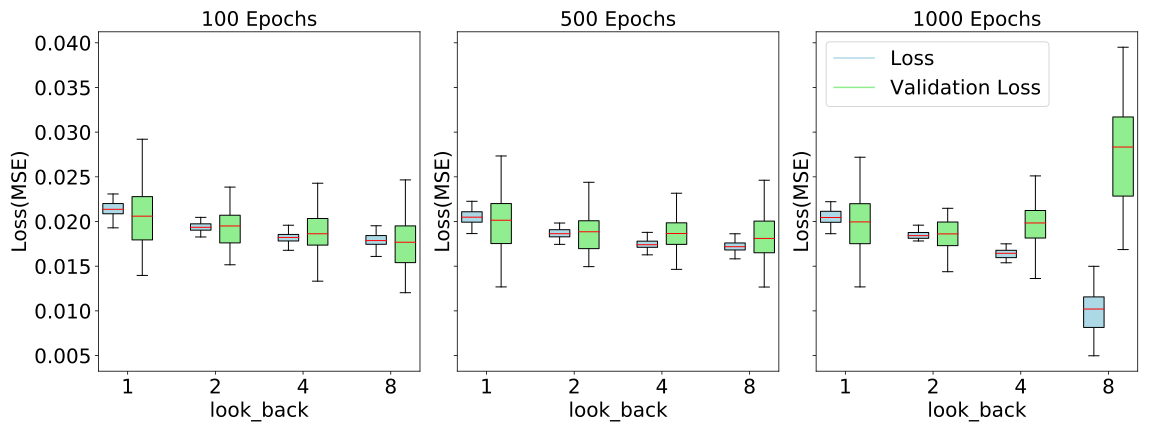
\includegraphics[width=1\linewidth]{Pictures/Results/experiment_2_1_1}
	\caption{The loss and validation loss when increasing the number of previous values to take into 
		account for a prediction for pair (1,11).}
	\label{fig:experiment_2}
\end{figure}

\paragraph{Number of Batches}
In Keras the parameter that controls the number of batches is called \textit{batch\_size}, this parameter indirectly controls the size of the batches by defining how many batches are created.
So, through increasing the number of batches (fewer values per batch) in Figure \ref{fig:experiment_4}, it is clear that with smaller batches you need a much higher number of epochs to get the same result.
This occurs because in each epoch only one randomly chosen batch is shown to the model for training, so to get an equal coverage of the data it takes more epochs.
The plots show that at some point smaller batches perform at least as good as the one big batch, but a lot more epochs are needed.
However, one big batch also takes a lot longer to compute than one small batch per epoch, so a trade-off has to be found between computation time per epoch and number of epochs.
\begin{figure}
	\centering
	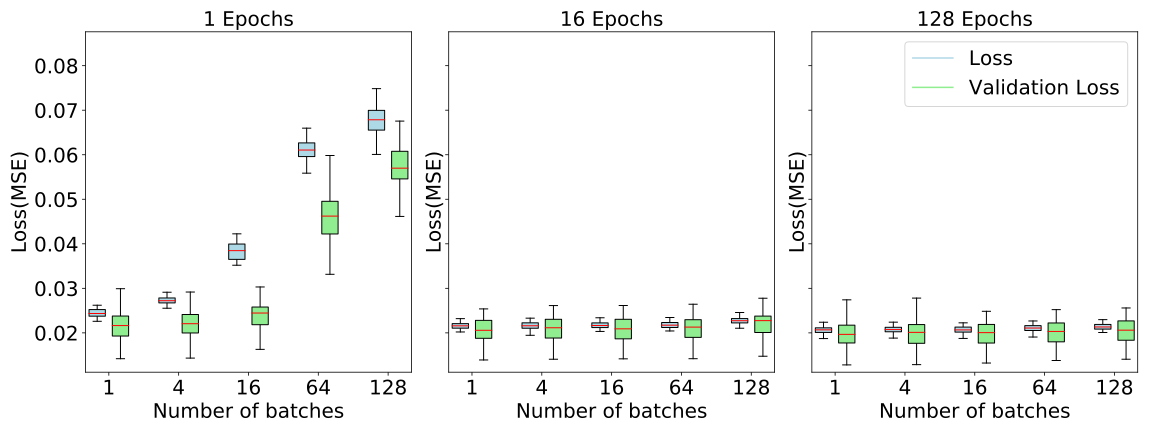
\includegraphics[width=1\linewidth]{Pictures/Results/experiment_4_1}
	\caption{The impact of epochs vs. number of batches for pair (1,11).}
	\label{fig:experiment_4}
\end{figure}

\paragraph{LSTM Layers}
The last parameter tested was how the number of LSTM layers influence the prediction error; the layers are stacked just like in Figure \ref{fig:unrolled2layerlstm}.
The plot in Figure \ref{fig:experiment_3} shows that more layers only slightly improve the predictions and and this is not the case for the other pairs (Figure \ref{fig:experiment_3_2} to Figure \ref{fig:experiment_3_5}).
This advantage also disappears further, when increasing the number of training epochs beyond 100.
These plots show that in this application, the number of layers is playing a small role and one can completely disregard it when using enough epochs.
This could be because the extra layers have the same number of hidden nodes in them like the previous ones and perform predictions based on predictions with the same complexity in each layer.
A possible improvement could be the increase in complexity in the extra layers.

\begin{figure}
	\centering
	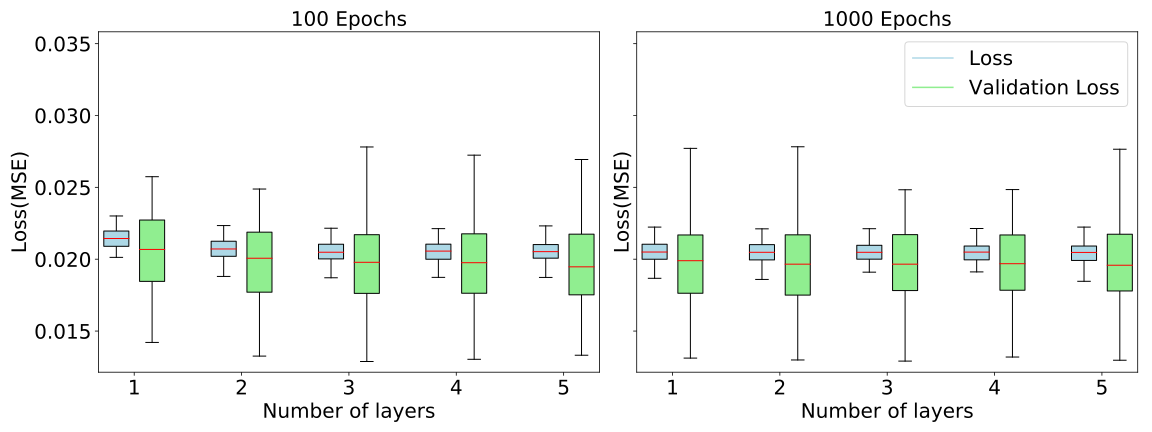
\includegraphics[width=1\linewidth]{Pictures/Results/experiment_3_1}
	\caption{Plot of how the number of LSTM layers influence the loss and validation loss for pair (1,11).}
	\label{fig:experiment_3}
\end{figure}

Now using all the test results, I can build a model that can predict the traffic.
Since the test results were so similar, even one hyperparameter setting could work for all communication pairs.
The plots in Figure \ref{fig:experiment_3} show that the model can use only one layer without it harming the predictions.
The exception for this is the first communication pair.
To get an equally good prediction for the first pair the number of epochs is chosen to be 1000.
Also, the high number of epochs has only a negative effect when the model uses more than two previous values (look\_back in the plot) , so the look\_back is going to be two for the model.
To speed up the training, since the model is training with 1000 epochs, I chose a batch size of 128.
Furthermore, only one hidden node is selected, as more nodes do not bring an advantage.

Using this model trained for 1000 epochs produces results that Figure \ref{fig:LSTMpredictions} shows.
The rest can be seen in the Appendix in Figure \ref{fig:LSTMprediction_0} to \ref{fig:LSTMprediction_4}.
The test set contains the 200 most current values, and the models have never seen these values.
The results vary from very good prediction (Figure \ref{fig:LSTMprediction_03}) to bad predictions (Figure \ref{fig:LSTMprediction_01}).
What the results seem to have in common is that they are good at predicting the rough shape of the traffic.
What all seem to struggle with is to get the exact values correct.      

\begin{figure}
	\centering
	\begin{subfigure}{1\linewidth}
		\centering
		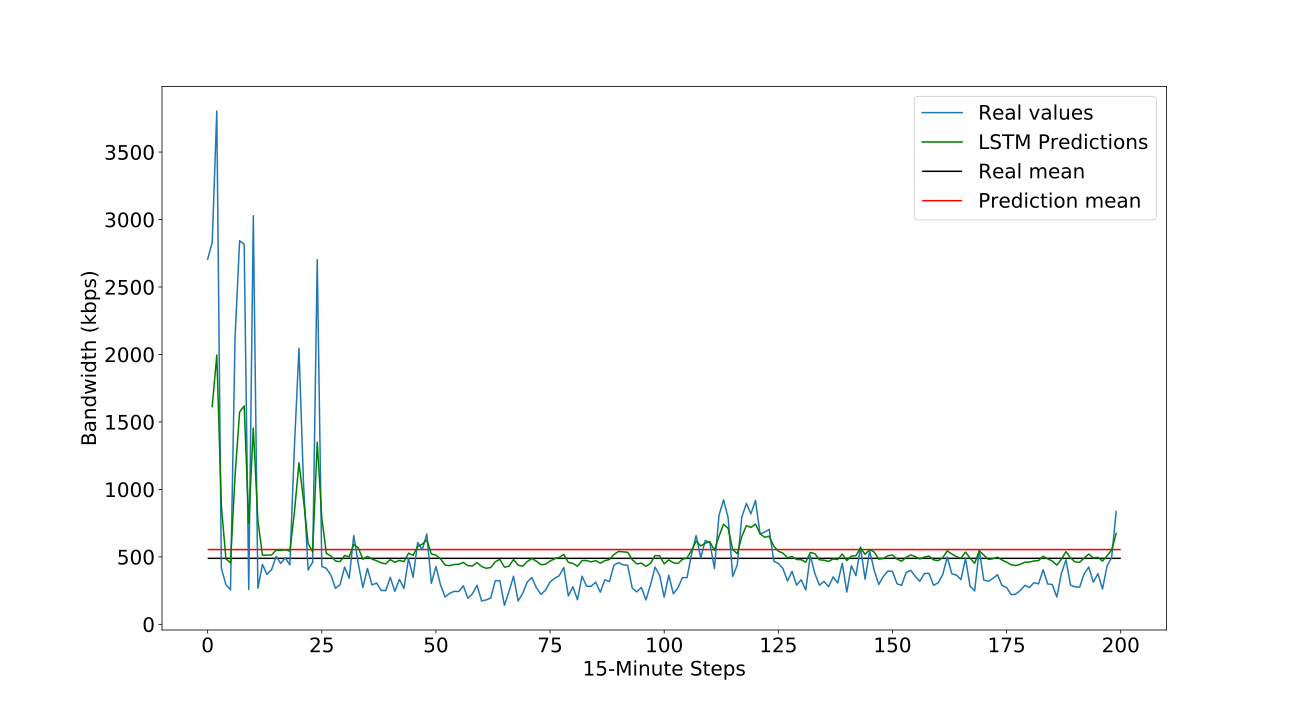
\includegraphics[width=1\linewidth]{Pictures/Practical_Examples/LSTMprediction_1}
		\caption{Pair (2, 11)}
		\label{fig:LSTMprediction_01}
	\end{subfigure}
	\begin{subfigure}{1\linewidth}
		\centering
		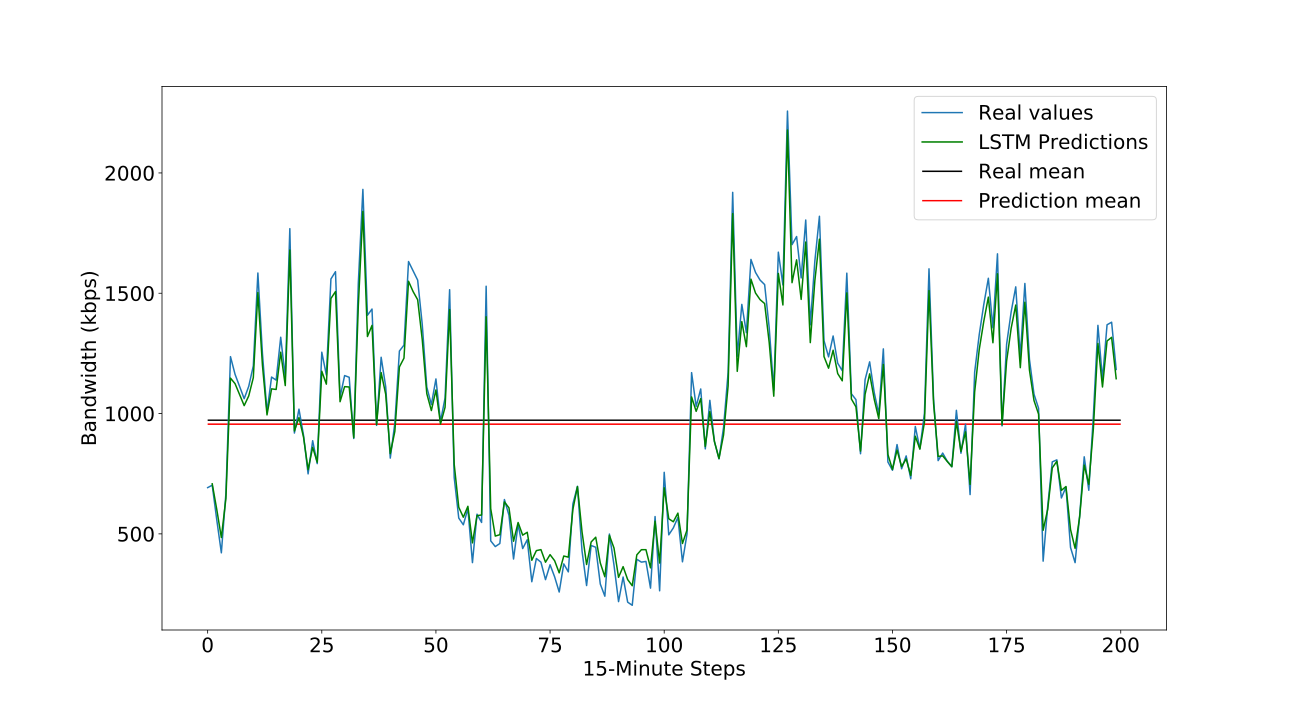
\includegraphics[width=1\linewidth]{Pictures/Practical_Examples/LSTMprediction_3}
		\caption{Pair (4, 11)}
		\label{fig:LSTMprediction_03}
	\end{subfigure}
	\caption{Prediction results of the traffic of pair (2,11) and (4,11).}
	\label{fig:LSTMpredictions}
\end{figure}

\subsection{The ARIMA Model}
Since I used the automatic ARIMA model builder, in this section, a short description is given on how the different chosen models look.

The values in the table below show the orders of the parts of the ARIMA model, chosen by the automatic ARIMA optimization.    

\begin{center}
	\begin{tabular}{|c|c|c|c|c|c|c|}
		\hline 
		source & p & d & q & P & D & Q \\ 
		\hline 
		1 & 1 & 1 & 2 & 0 & 0 & 0 \\ 
		\hline 
		2 & 3 & 0 & 3 & 2 & 0 & 1 \\ 
		\hline 
		3 & 2 & 0 & 2 & 0 & 0 & 0 \\ 
		\hline 
		4 & 1 & 1 & 2 & 0 & 0 & 1 \\ 
		\hline 
		5 & 3 & 0 & 3 & 2 & 0 & 2 \\ 
		\hline 
	\end{tabular}
\end{center}

When using these automatically optimized models two of the predictions of those models can be seen in Figure \ref{fig:ARIMAprediction1}, the rest can be seen in the Appendix in Figure \ref{fig:ARIMAprediction_0} to \ref{fig:ARIMAprediction_3}.
On first glance, these predictions look very similar to the LSTM predictions.
Of course, there exist some obvious errors that the LSTMs are not producing like the overcompensation in Figure \ref{fig:ARIMAprediction_4} at the 175th step.
Nevertheless, the models predict other parts of the traffic equally well.

\subsection{Comparing LSTM and ARIMA}    
Comparing all the errors from the ARIMA and the LSTM, the similarity in performance is undeniable.
Figure \ref{fig:BoxERRORprediction} shows the average error in the predictions of the test set.
Overall the LSTM is not much better than the ARIMA model.
What could be said, is that the LSTM is more consistent as it produces fewer outliers than the ARIMA.

\begin{figure}
	\begin{subfigure}{1\linewidth}
		\centering
		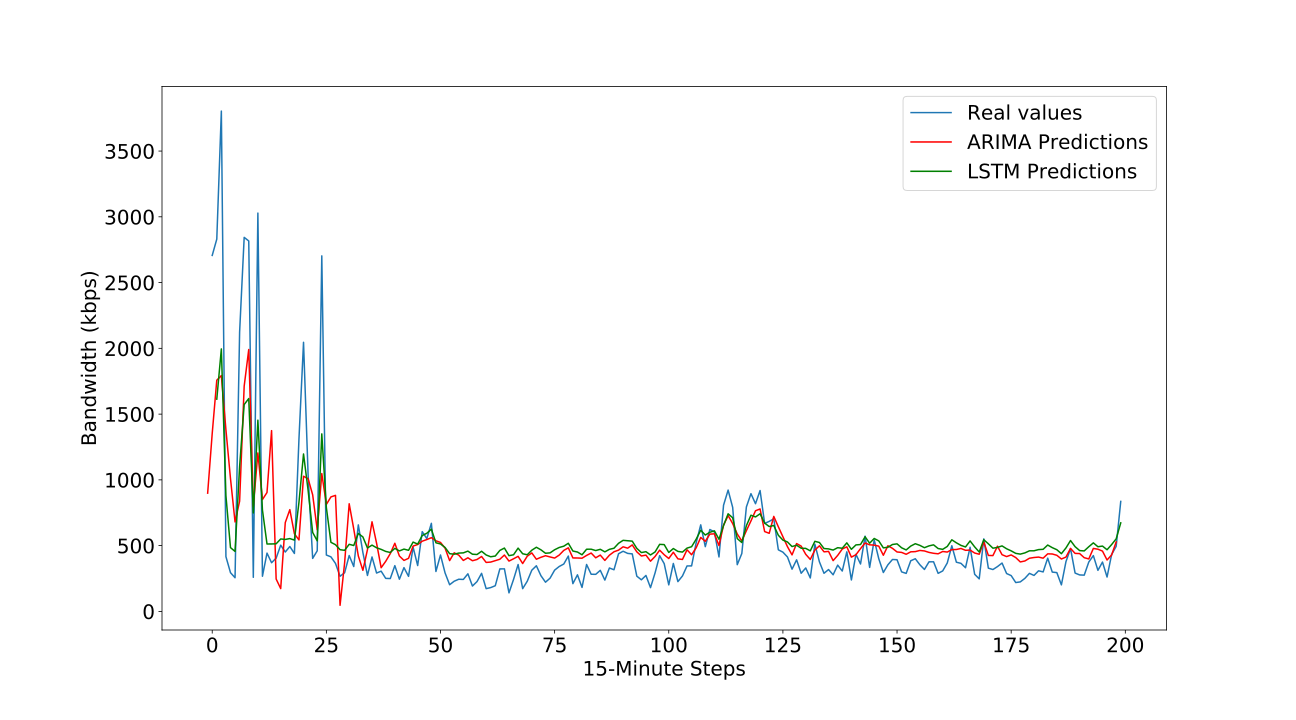
\includegraphics[width=1\linewidth]{Pictures/Practical_Examples/AvLprediction_1}
		\caption{Pair (2, 11)}
		\label{fig:ARIMAprediction_1}
	\end{subfigure}
	\begin{subfigure}{1\linewidth}
		\centering
		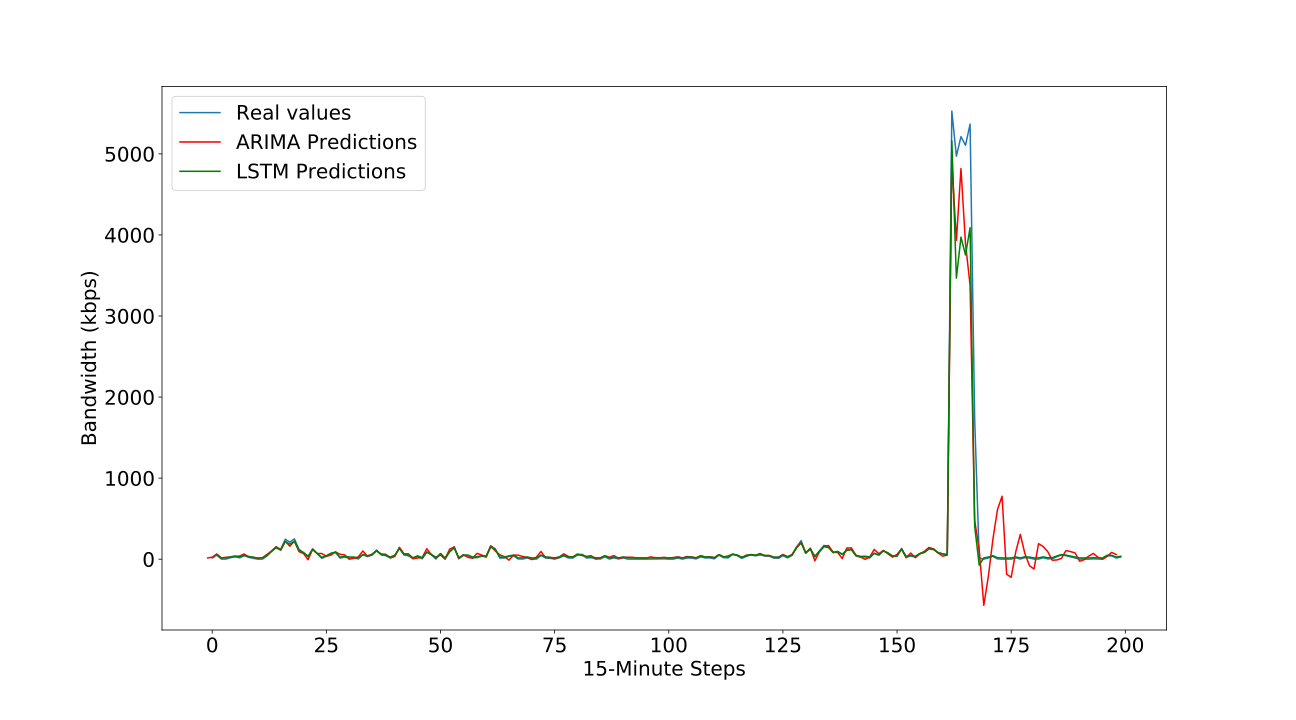
\includegraphics[width=1\linewidth]{Pictures/Practical_Examples/AvLprediction_4}
		\caption{Pair (5, 11)}
		\label{fig:ARIMAprediction_4}
	\end{subfigure}
	\caption{Predictions of the ARIMA model vs the LSTM model.}
	\label{fig:ARIMAprediction1}
\end{figure}

\begin{figure}
	\centering
	\begin{subfigure}{0.42\linewidth}
		\centering
		\includegraphics[width=1\linewidth]{Pictures/Practical_Examples/BoxERRORprediction_0}
		\caption{Pair (1, 11)}
		\label{fig:BoxERRORprediction_0}
	\end{subfigure}
	\begin{subfigure}{0.42\linewidth}
		\centering
		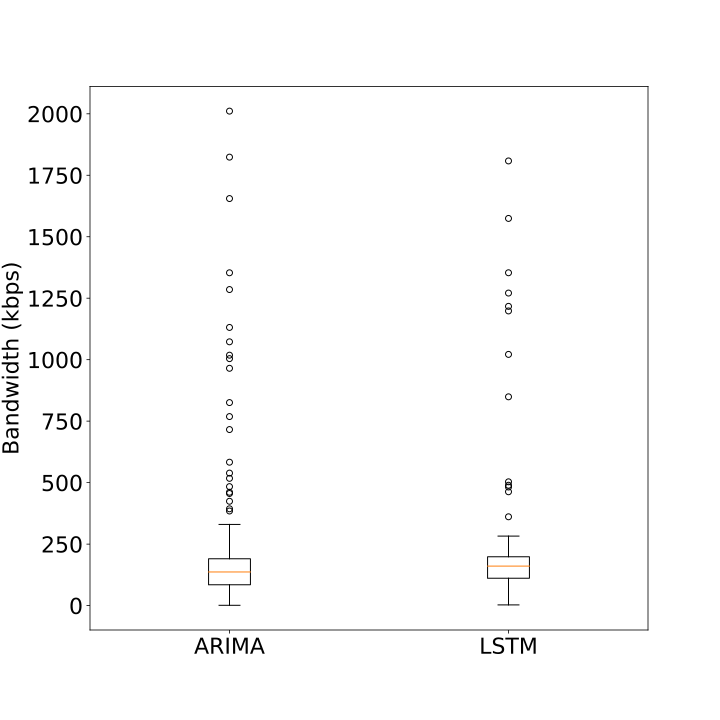
\includegraphics[width=1\linewidth]{Pictures/Practical_Examples/BoxERRORprediction_1}
		\caption{Pair (2, 11)}
		\label{fig:BoxERRORprediction_1}
	\end{subfigure}
	\begin{subfigure}{0.42\linewidth}
		\centering
		\includegraphics[width=1\linewidth]{Pictures/Practical_Examples/BoxERRORprediction_2}
		\caption{Pair (3, 11)}
		\label{fig:BoxERRORprediction_2}
	\end{subfigure}
	\begin{subfigure}{0.42\linewidth}
		\centering
		\includegraphics[width=1\linewidth]{Pictures/Practical_Examples/BoxERRORprediction_3}
		\caption{Pair (4, 11)}
		\label{fig:BoxERRORprediction_3}
	\end{subfigure}
	\begin{subfigure}{0.42\linewidth}
		\centering
		\includegraphics[width=1\linewidth]{Pictures/Practical_Examples/BoxERRORprediction_4}
		\caption{Pair (5, 11)}
		\label{fig:BoxERRORprediction_4}
	\end{subfigure}
	\caption{Comparison of the error in the prediction. ARIMA vs LSTM.}
	\label{fig:BoxERRORprediction}
\end{figure}

Also crucial for practical usage of the prediction models is how long they take to train and to predict a value.
This dictates how often the system can make a prediction and how fast an algorithm could react to future changes in the traffic.
Figure \ref{fig:BoxTraining} shows the times for training an LSTM model and fitting an ARIMA model.
The fitting of the ARIMA model is a lot faster than the training of the LSTM model.
I trained the LSTM model with 1000 epochs, so using only 100 epochs would get the LSTM training time closer to the ARIMA time, but that could only be done if it would not impair the prediction quality.

The second plot, Figure \ref{fig:BoxPrediction}, shows the differences between how long it takes a model to predict one value.
Included in the ARIMA time is the fitting of the model with the next value, as it is not usable if the model is not updated.
Here the LSTM has a clear advantage to the ARIMA model.
This is the case because for the LSTM the prediction is just calculating a few formulas with the previously found weights.
For the ARIMA, on the other hand, it is not just the calculation of the formulas but the refitting of the model with the new data.

These two plots show that one has to make a careful choice.
If the LSTM model needs to be retrained often, because the pattern of the data changes a lot, than the ARIMA has the clear advantage.
Especially if the LSTM model would get more complicated, the time for training would increase.
However, if the model does not have to be updated often, the LSTM performs much better than the ARIMA.

\begin{figure}
	\centering
	\begin{subfigure}{0.4\linewidth}
		\centering
		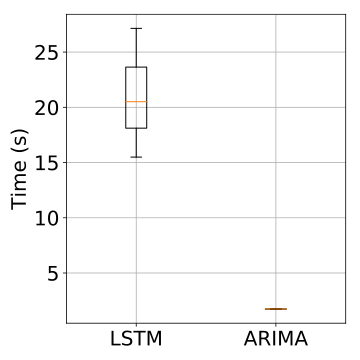
\includegraphics[width=1\linewidth]{Pictures/TimeComp/TrainingTime}
		\caption{The time needed for training/fitting the model}
		\label{fig:BoxTraining}
	\end{subfigure}
	\begin{subfigure}{0.4\linewidth}
		\centering
		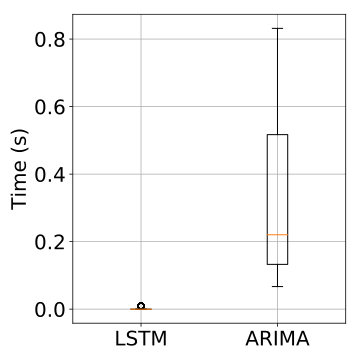
\includegraphics[width=1\linewidth]{Pictures/TimeComp/PredictionTime}
		\caption{The time needed for making a prediction of one value}
		\label{fig:BoxPrediction}
	\end{subfigure}
	\caption{Comparison of the relevant times measured for a LSTM and an ARIMA model}
	\label{fig:Times}
\end{figure}

With just these results, I cannot recommend using the LSTM over the ARIMA.
The performance on the prediction side is very similar, only decided by the lower number of outliers produced by the LSTM.
When looking at the time comparison, the LSTM is slower to train but faster at predicting values.
The only factor that distinguishes the two approaches is complexity.
One can automatically compute the ARIMA model after finding a suitable parameter m, number of periods in a season.
On the other hand, the LSTM model architecture allows for a vast number of different configurations and different parameter settings.
Finding the best parameters can also be done automatically via a hyperparameter optimization, but depending on the number of parameters and the computation resources available, the optimization can take up to a few days to complete.

\subsection{Optimizing LSTM Prediction}\label{optimization}
To analyze the predictions, I looked closer at the pair with the worst predictions, pair (2,11).
When looking at the prediction in Figure \ref{fig:LSTMprediction_01}, the predictions never go below a specific value.
Furthermore, the model predicts the majority of the values too high.
\begin{figure}
	\centering
	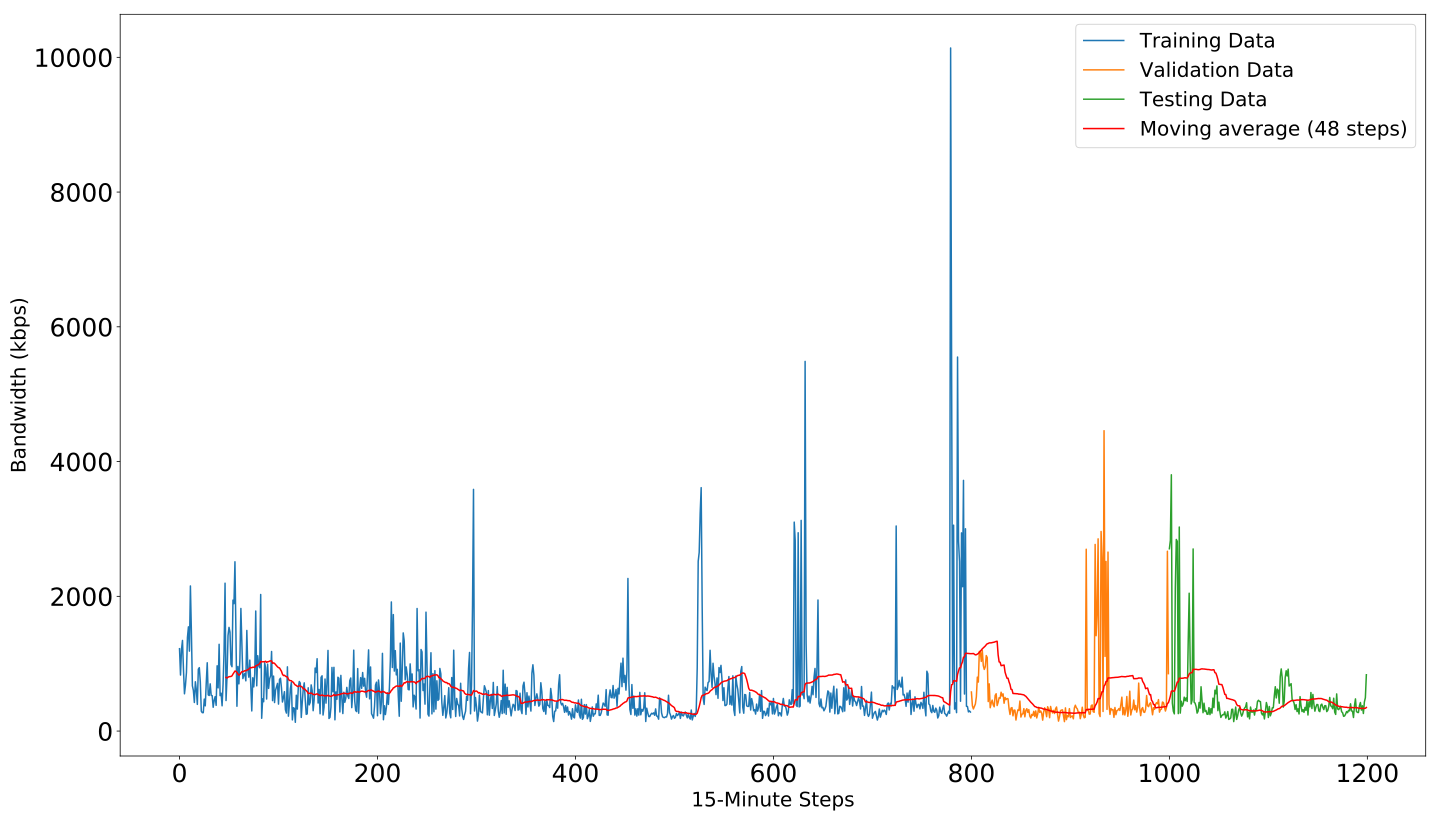
\includegraphics[width=0.95\linewidth]{Pictures/Traffic_Analysis/Traffic_rolling_average_2}
	\caption{The traffic from pair (2,11) used for training, validating and testing the model.}
	\label{fig:trafficrollingaverage2}
\end{figure}
Figure \ref{fig:trafficrollingaverage2} shows the traffic of the pair (2,11) and how it was split up into training, validation and testing data.
Also included in the Figure is the moving average over 48 steps, that is equivalent to 12 hours, so it is a 12-hour moving average.
In the first part of the data from step 0 to 400 the moving average shows a decline with two small spikes but no discernible pattern.
Looking further to the right after step 400, a pattern emerges.
There are bumps in the moving average of the length of roughly 100 steps.
The bumps continue until step 800 with a broader bump in the average.
After that broader bump, it continues with the spikes of width 100.
When seeing this pattern, maybe the prediction could be improved when omitting the first 400 steps that show no sign of the pattern.
Additionally, to omitting the 400 steps, the test includes multiple data ranges in 100 step steps, training with 100 steps, 200 steps and continuing this to 600 steps.
However, testing with the 600 steps that omit the 400 first steps has absolutely no influence on the prediction.
The model performs the same as with the 1000 steps.
What improved the model was training it with just 200 steps.
As can be seen in Figure \ref{fig:opti}, the predictions get closer to the actual real values.
This proves that the amount of training data fundamentally changes the ability of a model to make accurate predictions.
Also, this makes the models more challenging to use in a practical scenario as every model needs a different amount of data and a way of identifying how much data it needs.
What is also very important is that training the model with only 200 values made the training a lot more inconsistent.
The result in Figure \ref{fig:opti} is one of the better results, but the training could also result in a worse performance than training with the 1000 values.
\begin{figure}
	\centering
	\includegraphics[width=1\linewidth]{Pictures/optimization/LSTMoptimization_1_take2}
	\caption{Prediction when LSTM is trained with 200 values.}
	\label{fig:opti}
\end{figure}

\subsection{One-Step Prediction vs Multi-Step Prediction}
In this section two approaches are closer described that the ARIMA model can not replicate.
The first approach is the prediction of values more than one step in the future from the current value.
As mentioned earlier the ARIMA model can predict multiple values into the future at once, but anything beyond one value ahead has no usable accuracy.
Again using the example of the sequence [1,2,3,4,5], an example would be to predict the 4 based only on the sequence 1,2.
The training of the LSTM works the same as with the one-step prediction.
The input sequence stays the same, what changes are the target values.
These values are shifted by the number of values one wants to predict in the future.
\begin{figure}
	\centering
	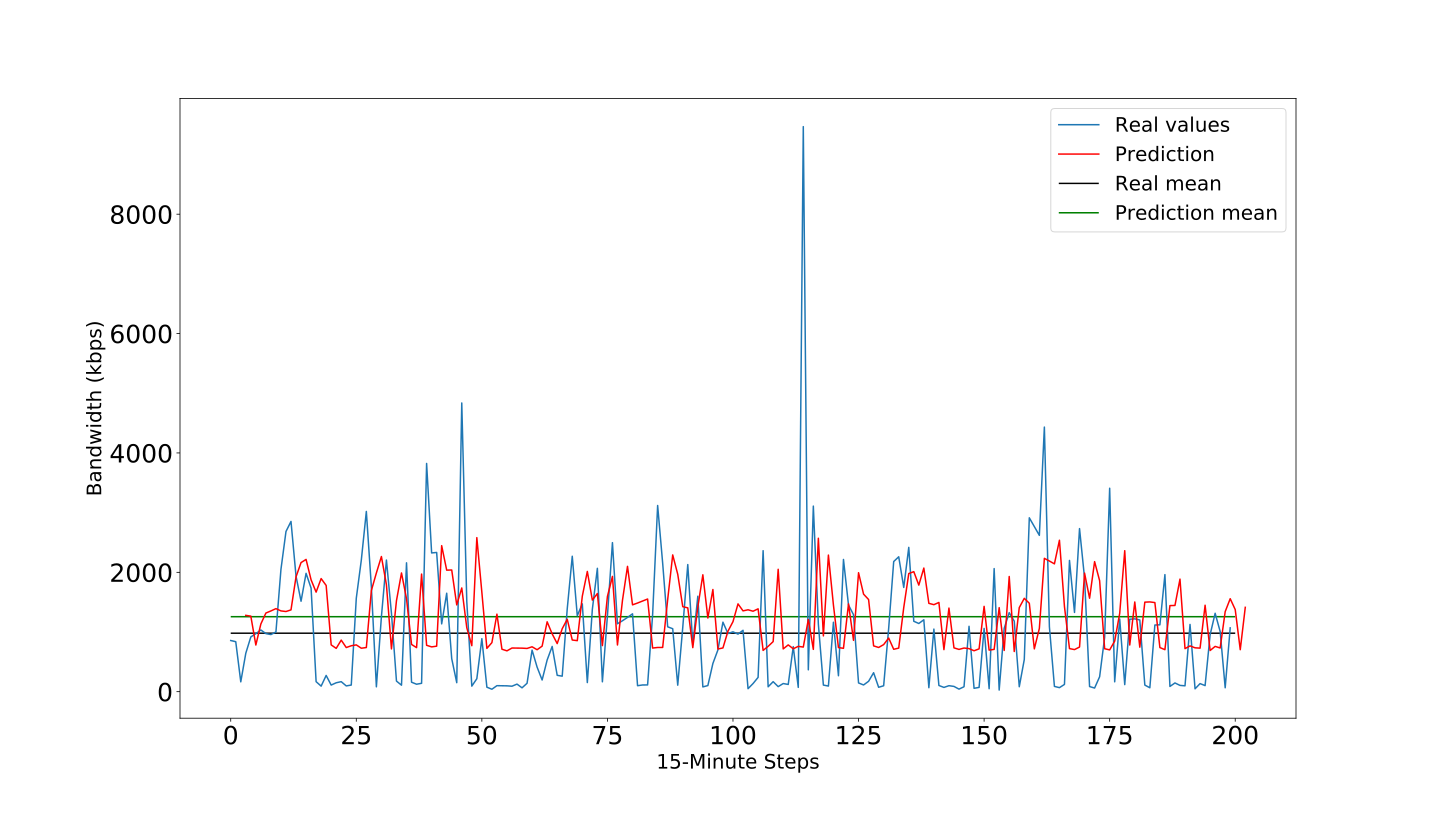
\includegraphics[width=1\linewidth]{Pictures/BigStep/LSTM_Big_Step_40}
	\caption{LSTM prediction, when trained with 4 steps into the future.}
	\label{fig:lstmbigstep0}
\end{figure}
But what happens when the LSTM is trained this way is displayed in Figure \ref{fig:lstmbigstep0}.
In this example the LSTM was trained to predict 4 values into the future with two previous values as input.
So, using two values to predict the next value in 4 steps.
But the LSTM not actually predicts the value in 4 steps but a shifted and squashed version of the next step.
So when inputting the value n-1 and n, instead of predicting n+4 the model predicted n+1 in a scaled down version.
This trend continues when predicting further into the future.
The squashing of the prediction continues until it approaches the mean of the one-step prediction.
In Figure \ref{fig:bigStep1} this trend can be observed as the prediction of 16 steps into the future represents the mean of the predictions one step into the future.

The same phenomenon can be observed when trying to teach the LSTM to predict a range of future values instead of just one value; for example predict the next five values.
When taking the output of each prediction that should represent n+1, n+2, n+3 and so forth and plotting them all on the nth step the output looks like in Figure \ref{fig:lstmrange1}.
The example predicted the 10 next values, only using the two previous values.
But here the output also produces multiple versions of the same function, which are more squashed the further into the future the prediction lies.
\begin{figure}
	\centering
	\begin{subfigure}{1\linewidth}
		\centering
		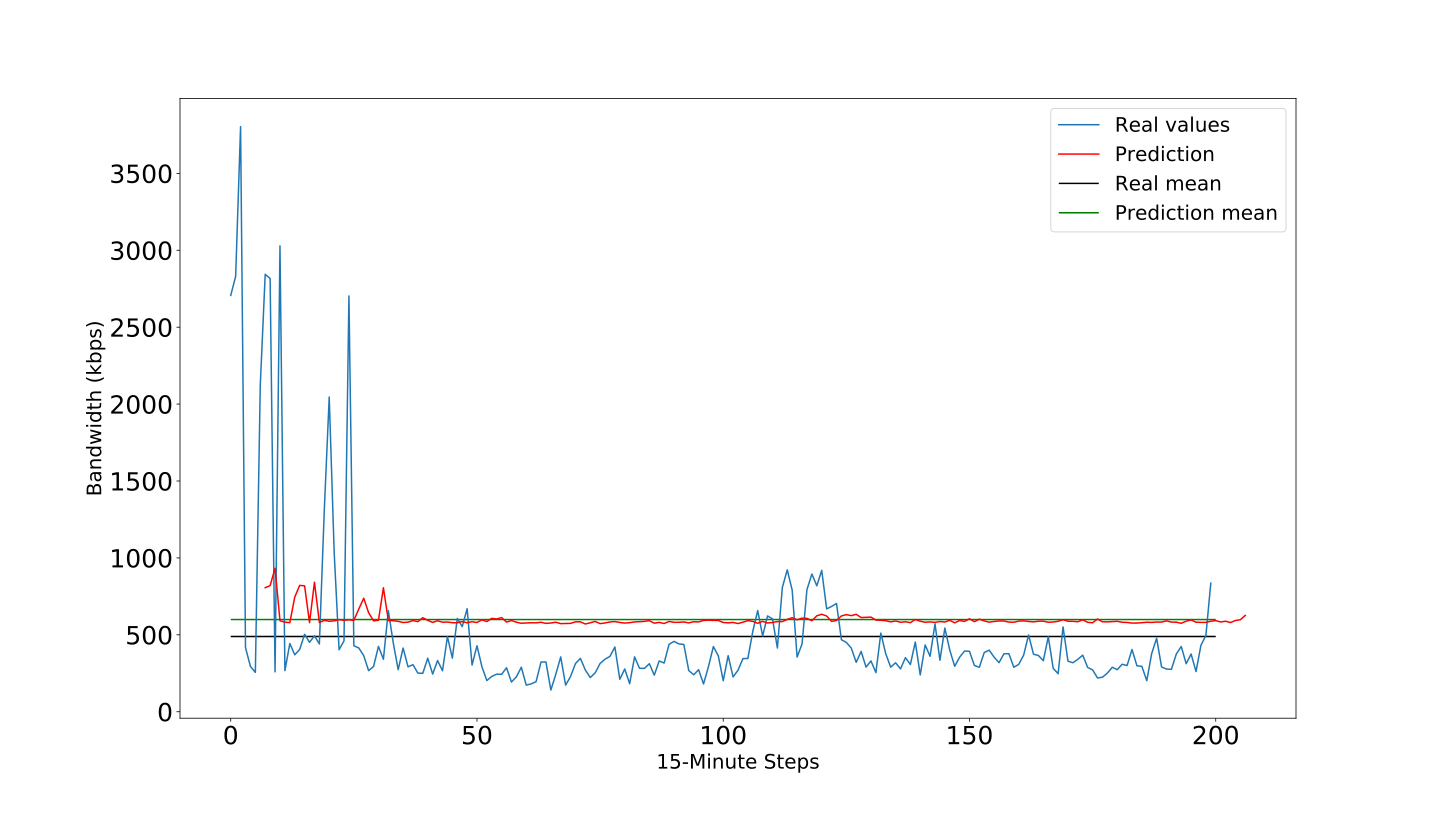
\includegraphics[width=1\linewidth]{Pictures/BigStep/LSTM_Big_Step_81}
		\caption{8 Steps into the future}
		\label{fig:bigStep8}
	\end{subfigure}
	\begin{subfigure}{1\linewidth}
		\centering
		\includegraphics[width=1\linewidth]{Pictures/BigStep/LSTM_Big_Step_161}
		\caption{16 Steps into the future}
		\label{fig:bigStep16}
	\end{subfigure}
	\caption{The prediction of an LSTM predicting 8 and 16 steps into the future.}
	\label{fig:bigStep1}
\end{figure}

\begin{figure}
	\centering
	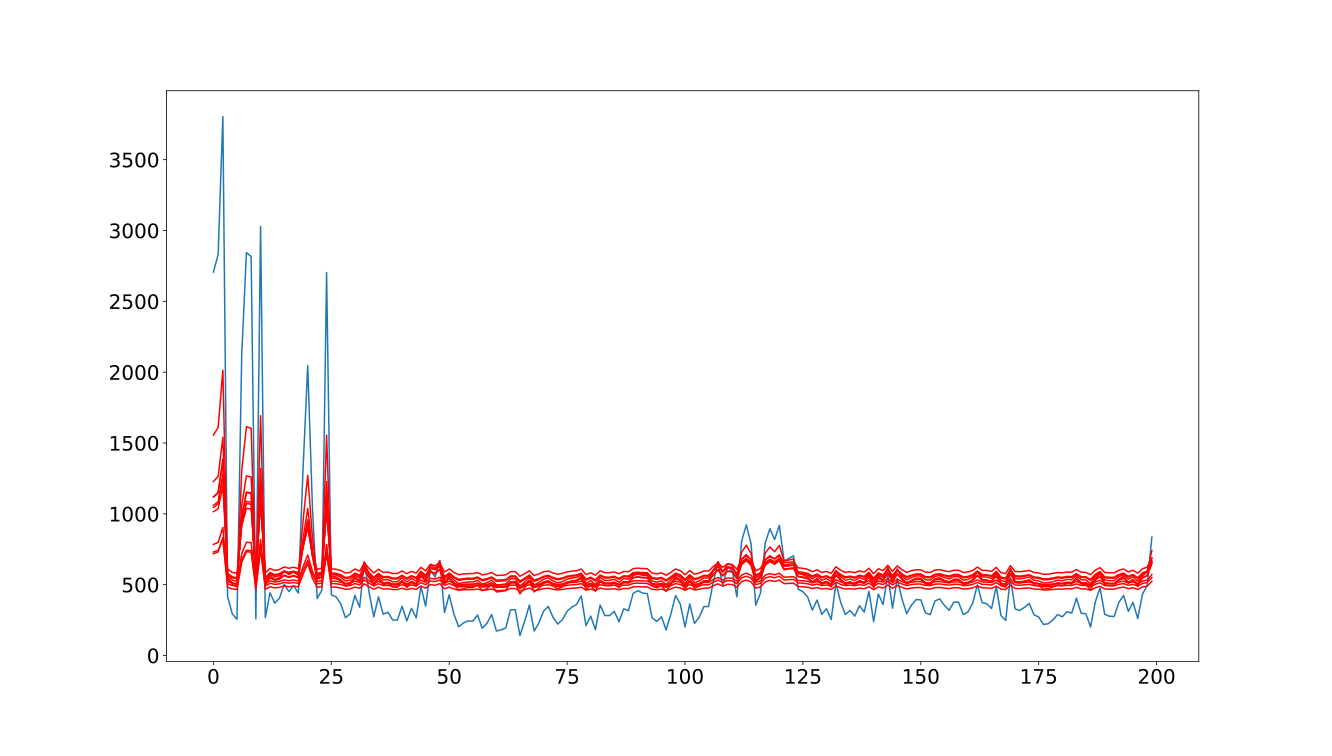
\includegraphics[width=1\linewidth]{Pictures/RangePrediction/LSTM_Range_1}
	\caption{10 values predicted at the same time plotted without shift.}
	\label{fig:lstmrange1}
\end{figure}

	
	%\pagebreak
	
	\section{Future Work and Conclusion}
This last section describes possible approaches for building upon the results of this thesis.
Furthermore, it analyzes and sums up the outcomes. 
\subsection{Future Work}
One of the biggest possible additions to this thesis is testing the results on a live system.
The live system would be perfect to find out how often the user has to retrain the Long Short-Term Memory model or how often the user has to initialize a new Auto-Regressive Integrated Moving Average model.
When recording the live network traffic, the traffic can be put directly into the models and one can compare the predictions directly to the real traffic.
Also, when putting this predicted traffic directly into a Virtual Network Function scaling and placing algorithm, the behaviour of the algorithm can be analyzed.
This behaviour can then lead to first estimates what actual errors are acceptable and at what value the error is growing too big.

Since the performance of the LSTM was so similar to the ARIMA model, one should try to analyze other RNN layers.
Keras supports GRU (Gated Recurrent Units) and ConvLSTM2D (Convolutional LSTM 2-Dimensional) layers.
The works \cite{8717800} \cite{8292737}, already mentioned in the Related Work chapter, both successfully use convolutional RNNs.

Additionally, on-the-fly-learning could be a promising strategy.
When using each new step to directly continue the training of the model, the retraining of the model could possibly be eliminated.
However, one would have to check if a training step after each new value is the optimal way or if the system has to wait until a whole new batch is complete.
When using this approach, other layers likely have to be included in the model.
I surmise that, because the system trains the model with much more data, a dropout layer would have to be included to prevent overfitting.
A dropout layer drops some of the data that passes through it: how much data the layer is dropping can be configured.
Furthermore, other layers also have a dropout parameter (the LSTM layer, for example).
This would have to be included in the experiments as well.

Additionaly the size of the steps may play a role in the prediction quality.
The Abilene set \cite{SNDlib10}, \cite{OrlowskiPioroTomaszewskiWessaely2010}, has just 5-Minute steps.
Maybe the 15-Minute steps have less correlation as they pack more data into one step.
That should also be tested and in a live system the step size could be chosen arbitrarily.
Also a point that calls for tests with a live system.


\subsection{Conclusion}
The goal of this thesis was to analyze if an Long Short-Term Memory model is a viable approach to predicting network traffic in a Network Function Virtualization scenario.
And this goal was fulfilled in part.
The prediction models work well.
When putting traffic in, a usable prediction for the next step can be achieved.
The predicted value can be interpreted in two parts: the change from the previously predicted value and the actual traffic value.
The reliable part of the prediction is the shape of the prediction, does the traffic go up or down in relation to the previously predicted value.
With this prediction the VNF scaling algorithm should be able to correctly scale the VNFs in the correct direction, up or down.
The other part of the prediction the actual network traffic causes the problems.
Depending on the traffic pattern the actual predicted level of traffic can be off of the actual level.
So, when putting an LSTM model before the placing and scaling algorithm it will be able to work with traffic predicted one step into the future.
With these predictions the scaling of the Virtual Network Functions will go in the correct direction, but depending on the traffic pattern the predicted traffic bandwidth will be wrong.
However, all these statements are also true for an Auto-Regressive Integrated Moving Average model.
With these results it should not matter, for the VNF scaling algorithms, if an LSTM or ARIMA model is used.
Maybe with additional test in different scenarios, as described in the previous section, a clear destinction can be made.

With these results I conclude that traffic prediction is a viable solution for NFV scenarios.
Not neccessarily a deep learning approach like an LSTM but ARIMA models can already greatly improve VNF scaling and placing algorithms.
The reuslts show that these algorithms can be changed from reactive to proactive with machine learning models.
	
	%\pagebreak

	\section{Appendix}

\subsection{Documents and Code}
In addition to the thesis document, python code is also part of this master's thesis.
The main library is the \textit{TimeSeriesModelCreator\_Parallel\_talos.py} file. This can be used to create LSTM prediction models.

Examples of the usage of the library can be found in the experiment files. An example is experiment one.

\begin{scriptsize}
\begin{lstlisting}
#!/usr/bin/env python

from TimeSeriesModelCreator_Parallel_talos import
	TimeSeriesModelCreator_Parallel_talos
import pandas as pd
import matplotlib.pyplot as plt

look_backs = [1]
modelCreators = []
for look_back in look_backs:
	modelCreators.append(TimeSeriesModelCreator_Parallel_talos
	(look_back,
	r'..\Datasets\GEANTCombined\all_in_one_complete_appended.csv'))

for modelCreator in modelCreators:
	batch_sizes = [100]
	epochs = [100,250,500,750,1000]
	nodes = [1, 2, 3, 8, 16, 32, 64, 128]
	layers = [1]
	optimizers = ['adam']
	losses = ['mean_squared_error']
	modelCreator.test_for_optimal_config('Epxeriment_1_1', 1, 5, 11, 11,
		1000, batch_sizes, epochs, nodes, layers, optimizers, losses,
		40,	1, 0, 200)
\end{lstlisting}
\end{scriptsize}

This is an example for testing multiple parameter variations.
From the results of this optimization a model can be created and the model is saved in the library object. Where it can be called using its name.
An example for this can be found in the Jupyter notebooks comparing the LSTM and the ARIMA models.
The following example creates five different models and uses them to predict traffic.

\begin{samepage}
\begin{scriptsize}
	\begin{lstlisting}
creator = TimeSeriesModelCreator_Parallel_talos(2,
	r'..\Datasets\GEANTCombined\all_in_one_complete_appended.csv')
modelMatch = {}
for x in range(1,6):
	creator.add_new_model(name = 'test'+str(x), nodes = 1, layer = 1, 
		loss='mean_squared_error', optimizer='adam')
	modelMatch[str(x)+'_11'] = 'test'+str(x)
	creator.train_model(1, 5, 11, 11, 1000, 200, modelMatch, 
		epoch = 1000, batch_size = 128, shift = 0)
	
LSTMpredictions = []
for x in range(1,6):
	prediction = creator.predict('test'+str(x), subsets_testing[x-1], 0)
	LSTMpredictions.append(prediction)
	\end{lstlisting}
\end{scriptsize}
\end{samepage}

These two examples cover most of the functionallities of the library. 
More examples and the library itself can be found in the \textit{source/Training} folder.

\subsection{Libraries and Frameworks}
\begin{itemize}
	\item Python 3.6.1
	\item Keras 2.2.5
	\item TensorFlow 1.14.0
	\item Talos 0.6.3
	\item Pandas 0.24.2
	\item sklearn 0.21.3
\end{itemize}

\subsection{Figures}
   
	\begin{figure}[H]
		\centering
		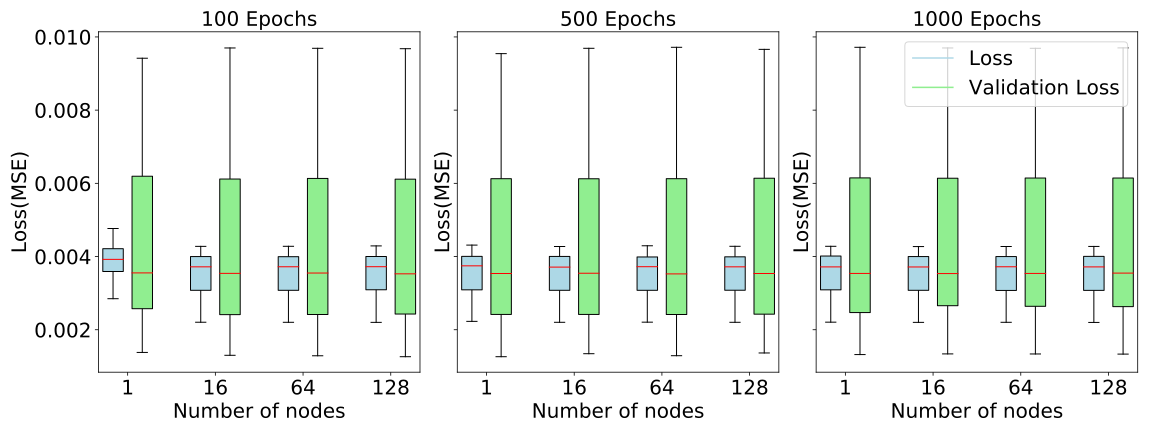
\includegraphics[width=1\linewidth]{Pictures/Results/experiment_1_1_2}
		\caption{The loss and validation loss when increasing the number of hidden nodes. Pair (2, 11)}
		\label{fig:experiment_1_1_2}
	\end{figure}
	\begin{figure}[H]
		\centering
		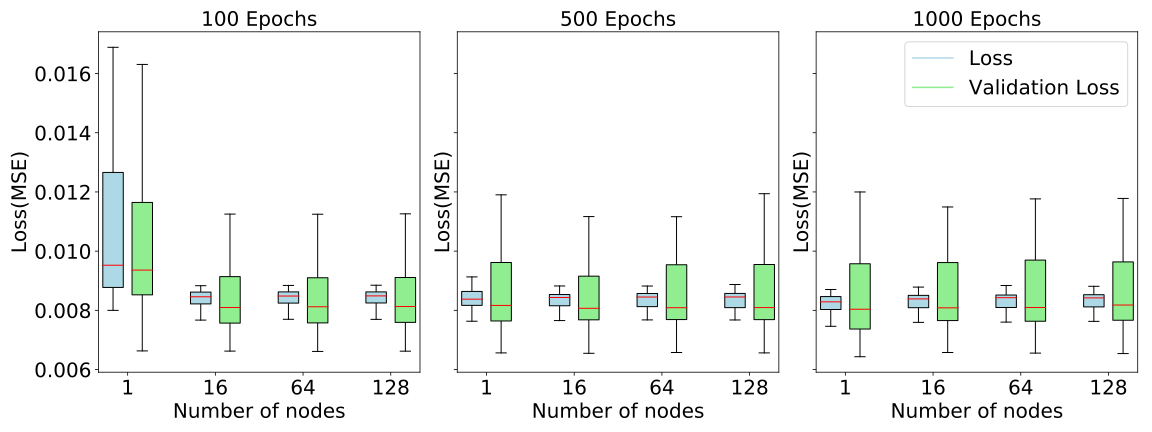
\includegraphics[width=1\linewidth]{Pictures/Results/experiment_1_1_3}
		\caption{The loss and validation loss when increasing the number of hidden nodes. Pair (3, 11)}
		\label{fig:experiment_1_1_3}
	\end{figure}
	\begin{figure}[H]
		\centering
		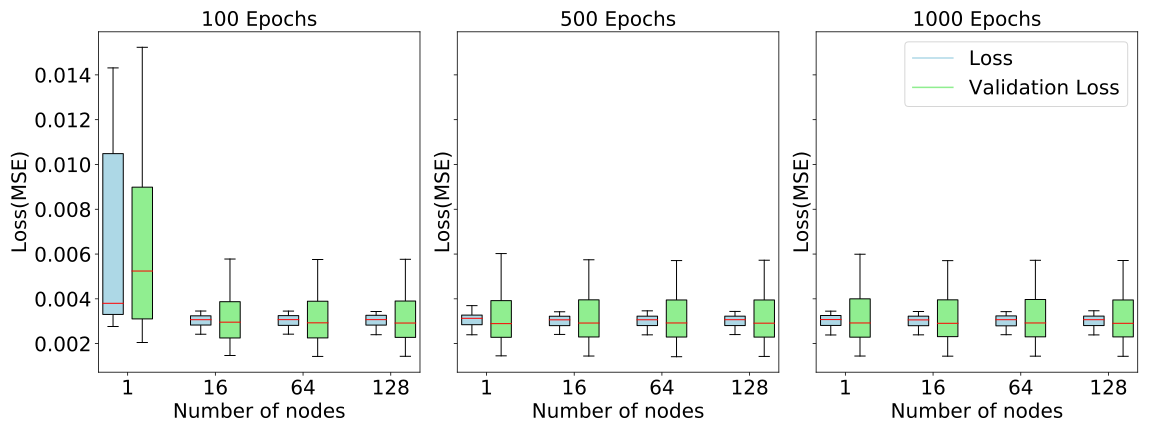
\includegraphics[width=1\linewidth]{Pictures/Results/experiment_1_1_4}
		\caption{The loss and validation loss when increasing the number of hidden nodes. Pair (4, 11)}
		\label{fig:experiment_1_1_4}
	\end{figure}
	\begin{figure}[H]
		\centering
		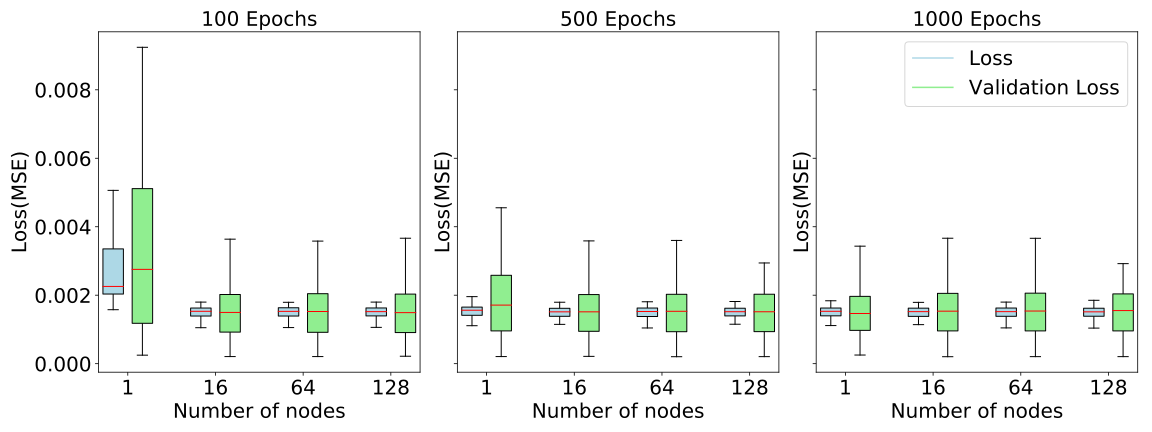
\includegraphics[width=1\linewidth]{Pictures/Results/experiment_1_1_5}
		\caption{The loss and validation loss when increasing the number of hidden nodes. Pair (5, 11)}
		\label{fig:experiment_1_1_5}
	\end{figure}


	\begin{figure}[H]
		\centering
		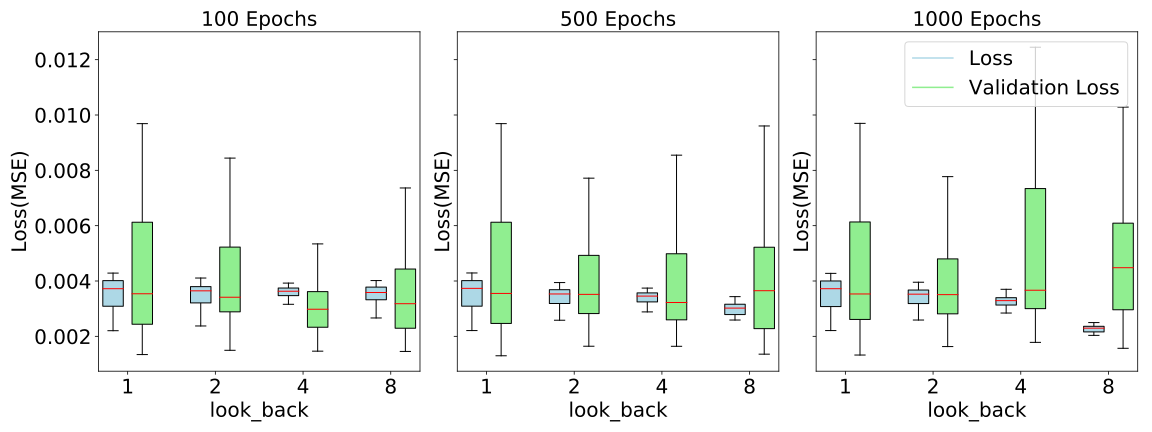
\includegraphics[width=1\linewidth]{Pictures/Results/experiment_2_1_2}
		\caption{The loss and validation loss when increasing the number of previous values to take into account for a prediction. Pair (2, 11)}
		\label{fig:experiment_2_1_2}
	\end{figure}
	\begin{figure}[H]
		\centering
		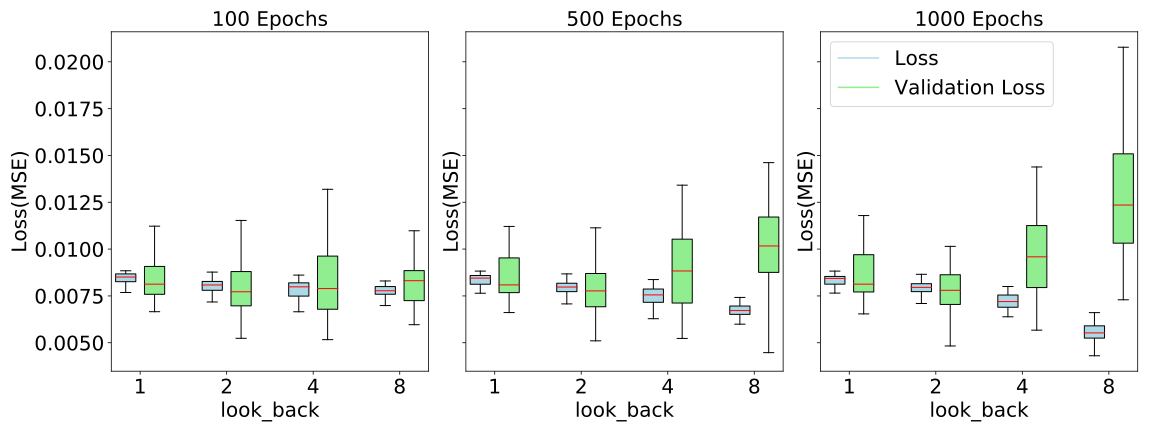
\includegraphics[width=1\linewidth]{Pictures/Results/experiment_2_1_3}
		\caption{The loss and validation loss when increasing the number of previous values to take into account for a prediction. Pair (3, 11)}
		\label{fig:experiment_2_1_3}
	\end{figure}
	\begin{figure}[H]
		\centering
		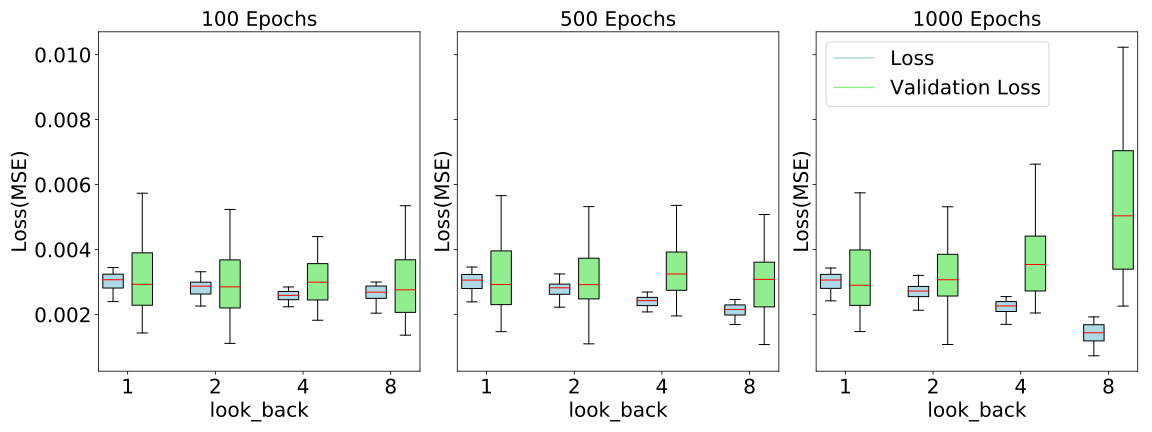
\includegraphics[width=1\linewidth]{Pictures/Results/experiment_2_1_4}
		\caption{The loss and validation loss when increasing the number of previous values to take into account for a prediction. Pair (4, 11)}
		\label{fig:experiment_2_1_4}
	\end{figure}
	\begin{figure}[H]
		\centering
		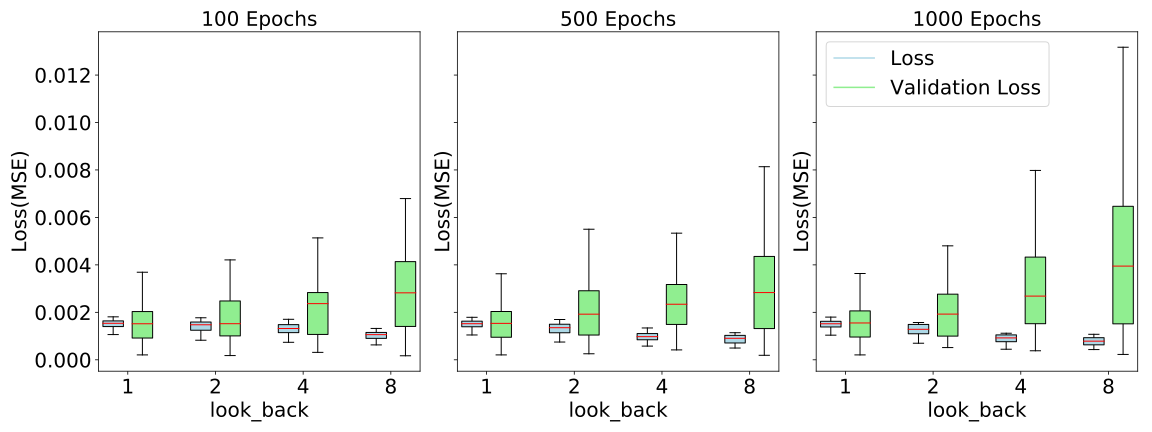
\includegraphics[width=1\linewidth]{Pictures/Results/experiment_2_1_5}
		\caption{The loss and validation loss when increasing the number of previous values to take into account for a prediction. Pair (5, 11)}
		\label{fig:experiment_2_1_5}
	\end{figure}


	\begin{figure}[H]
		\centering
		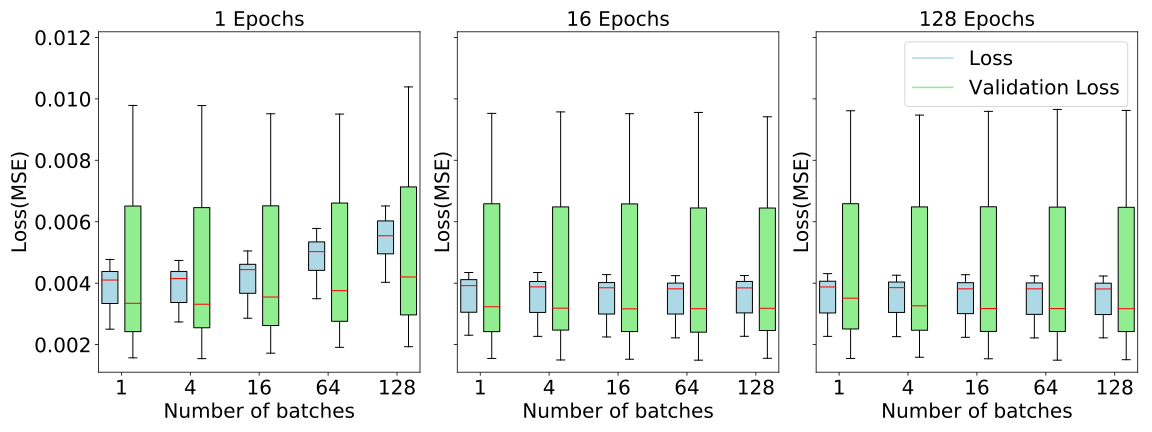
\includegraphics[width=1\linewidth]{Pictures/Results/experiment_4_2}
		\caption{The impact of epochs vs. number of batches. Pair (2, 11)}
		\label{fig:experiment_4_2}
	\end{figure}
	\begin{figure}[H]
		\centering
		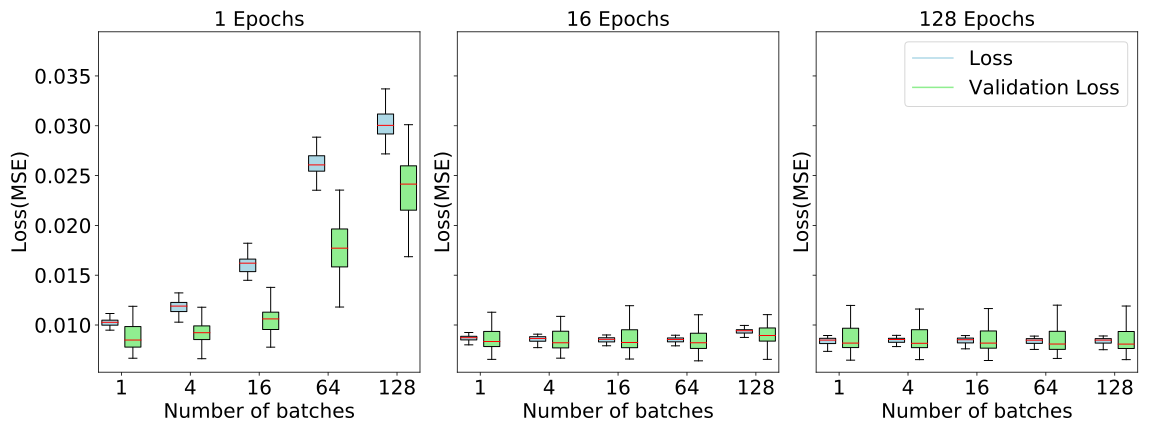
\includegraphics[width=1\linewidth]{Pictures/Results/experiment_4_3}
		\caption{The impact of epochs vs. number of batches. Pair (3, 11)}
		\label{fig:experiment_4_3}
	\end{figure}
	\begin{figure}[H]
		\centering
		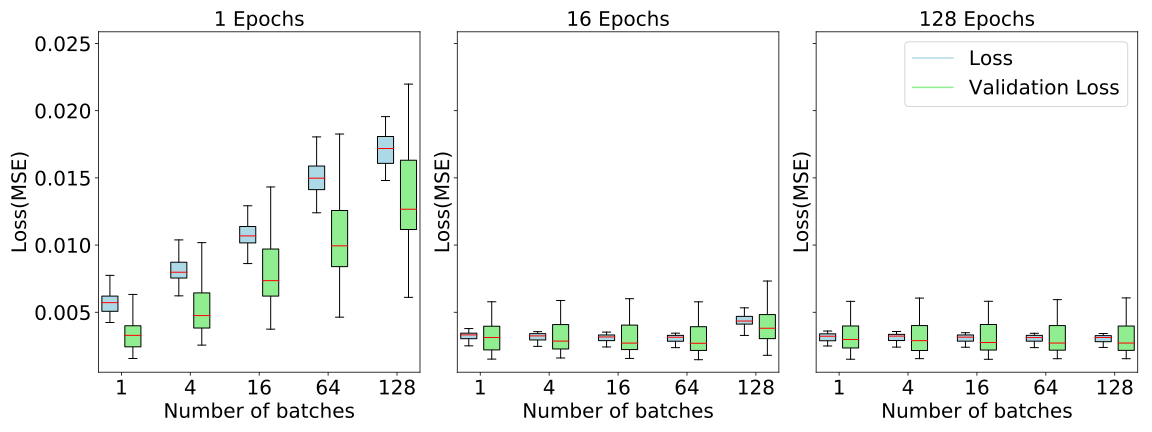
\includegraphics[width=1\linewidth]{Pictures/Results/experiment_4_4}
		\caption{The impact of epochs vs. number of batches. Pair (4, 11)}
		\label{fig:experiment_4_4}
	\end{figure}
	\begin{figure}[H]
		\centering
		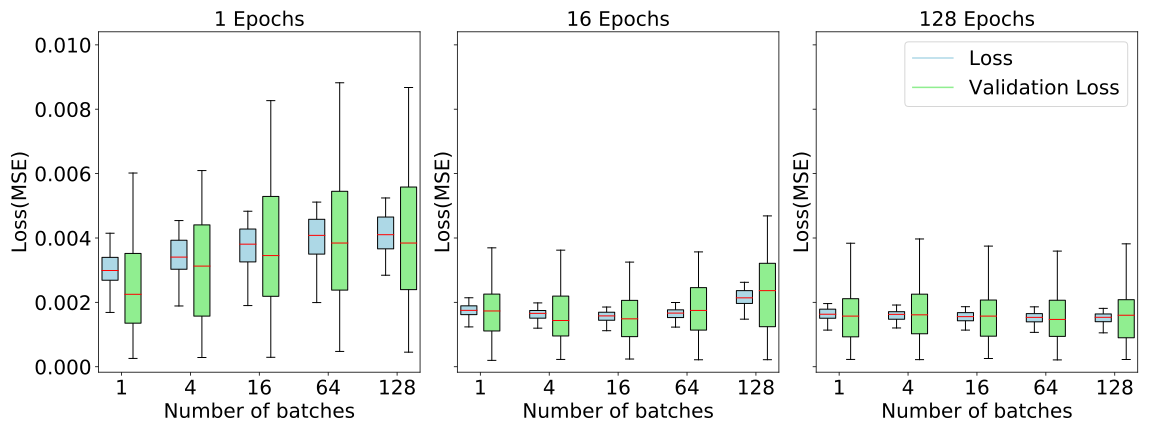
\includegraphics[width=1\linewidth]{Pictures/Results/experiment_4_5}
		\caption{The impact of epochs vs. number of batches. Pair (5, 11)}
		\label{fig:experiment_4_5}
	\end{figure}


	\begin{figure}[H]
		\centering
		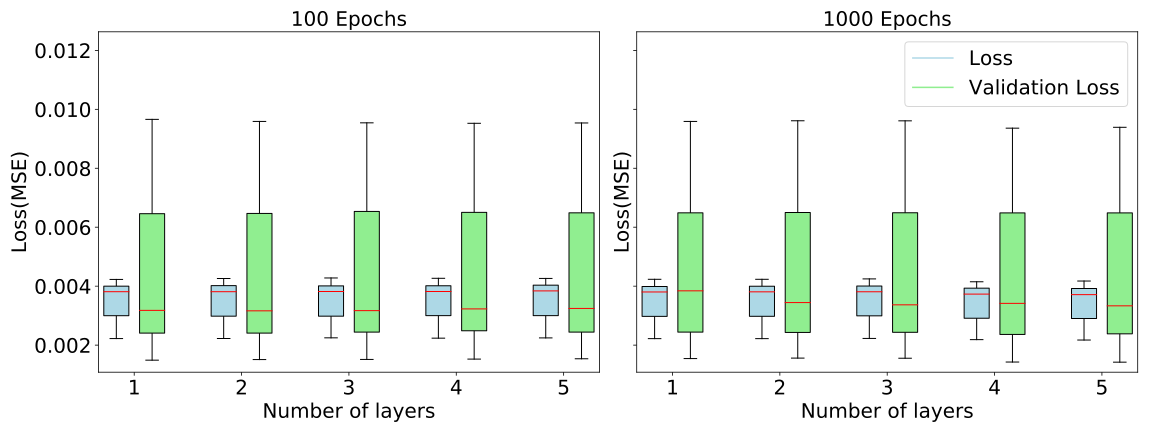
\includegraphics[width=1\linewidth]{Pictures/Results/experiment_3_2}
		\caption{Plot of how the number of LSTM layers influence the loss and validation loss. Pair (2, 11)}
		\label{fig:experiment_3_2}
	\end{figure}
	\begin{figure}[H]
		\centering
		\includegraphics[width=1\linewidth]{Pictures/Results/experiment_3_3}
		\caption{Plot of how the number of LSTM layers influence the loss and validation loss. Pair (3, 11)}
		\label{fig:experiment_3_3}
	\end{figure}
	\begin{figure}[H]
		\centering
		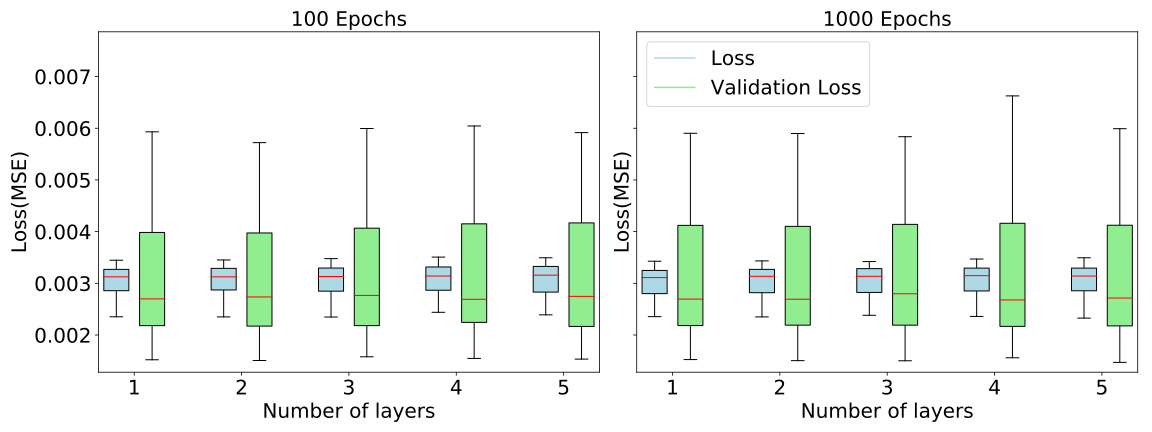
\includegraphics[width=1\linewidth]{Pictures/Results/experiment_3_4}
		\caption{Plot of how the number of LSTM layers influence the loss and validation loss. Pair (4, 11)}
		\label{fig:experiment_3_4}
	\end{figure}
	\begin{figure}[H]
		\centering
		\includegraphics[width=1\linewidth]{Pictures/Results/experiment_3_5}
		\caption{Plot of how the number of LSTM layers influence the loss and validation loss. Pair (5, 11)}
		\label{fig:experiment_3_5}
	\end{figure}


	\begin{figure}[H]
		\centering
		\includegraphics[width=1\linewidth]{Pictures/Practical_Examples/LSTMprediction_0}
		\caption{LSTM prediction of pair (1, 11)}
		\label{fig:LSTMprediction_0}
	\end{figure}
	\begin{figure}[H]
		\centering
		\includegraphics[width=1\linewidth]{Pictures/Practical_Examples/LSTMprediction_2}
		\caption{LSTM prediction of pair (3, 11)}
		\label{fig:LSTMprediction_2}
	\end{figure}
	\begin{figure}[H]
		\centering
		\includegraphics[width=1\linewidth]{Pictures/Practical_Examples/LSTMprediction_4}
		\caption{LSTM prediction of pair (5, 11)}
		\label{fig:LSTMprediction_4}
	\end{figure}


\begin{figure}[H]
		\centering
		\includegraphics[width=1\linewidth]{Pictures/Practical_Examples/AvLprediction_0}
		\caption{LSTM and ARIMA predictions of pair (1, 11)}
		\label{fig:ARIMAprediction_0}
\end{figure}
\begin{figure}[H]
		\centering
		\includegraphics[width=1\linewidth]{Pictures/Practical_Examples/AvLprediction_2}
		\caption{LSTM and ARIMA predictions of pair (3, 11)}
		\label{fig:ARIMAprediction_2}
\end{figure}
\begin{figure}[H]
		\centering
		\includegraphics[width=1\linewidth]{Pictures/Practical_Examples/AvLprediction_3}
		\caption{LSTM and ARIMA predictions of pair (4, 11)}
		\label{fig:ARIMAprediction_3}
\end{figure}

	%\pagebreak

	\bibliography{thesisBib}
	
	\pagebreak
		\section*{Selbständigkeitserklärung}
	Hiermit erkläre ich, dass ich die vorliegende Arbeit mit dem Titel\\
	\\
	\textbf{Machine Learning-Based Load Prediction for Network Function Virtualization Scenarios}\\
	\\
	selbstständig und ohne unerlaubte fremde Hilfe angefertigt, keine anderen als die angegebenen Quellen und Hilfsmittel verwendet und die den verwendeten Quellen und Hilfsmitteln wörtlich oder inhaltlich entnommenen Stellen als solche kenntlich gemacht habe.\\
	\\
	\\	
	
\begin{tabular}{@{}p{3.5in}p{4in}@{}}
	\hrulefill &\\
	Ort, Datum &\\
	&\\
	&\\
	\hrulefill &\\
	Unterschrift &\\
\end{tabular}
\end{document}